\documentclass[fleqn]{article}
\usepackage[UTF8]{ctex}
\usepackage{listings}
\usepackage{diagbox}
\usepackage[german]{babel}
\usepackage[T1]{fontenc}
\usepackage[latin1]{inputenc}
\usepackage{titlesec}
\usepackage{geometry}
\usepackage{qtree}
\usepackage{tikz}
\usepackage{amsmath}
\usepackage{amssymb}
\setcounter{secnumdepth}{0}
\usetikzlibrary{positioning}
\geometry{top=2.5cm, bottom=2.5cm}
\lstset{
 columns=fixed,       
 numbers=left,                                        % 在左侧显示行号
 numberstyle=\tiny\color{gray},                       % 设定行号格式
 frame=none,                                          % 不显示背景边框
 backgroundcolor=\color[RGB]{245,245,244},            % 设定背景颜色
 keywordstyle=\color[RGB]{40,40,255},                 % 设定关键字颜色
 numberstyle=\footnotesize\color{darkgray},           
 commentstyle=\it\color[RGB]{0,96,96},                % 设置代码注释的格式
 stringstyle=\rmfamily\slshape\color[RGB]{128,0,0},   % 设置字符串格式
 showstringspaces=false,                              % 不显示字符串中的空格
 language=c++,                                        % 设置语言
 breaklines,                                          % 自动换行
}

%\title{TU Chemnitz \\ Praktikum Grundlagen Technische Informatik \\ Versuch Sequ1}

%\author{Gruppe 5 - Team 5: \\ Dongze Yang \\Xiangyu Tong \\ Treshchun Kateryna}

\begin{document}

%\maketitle



\newpagestyle{main}{
    \sethead{}{}{Rechnernetze}
    \setfoot{}{\thepage}{}
    \headrule
    \footrule
}
\pagestyle{main}
\section{SS2018}

\noindent 3. Gegeben: 
\begin{center}
    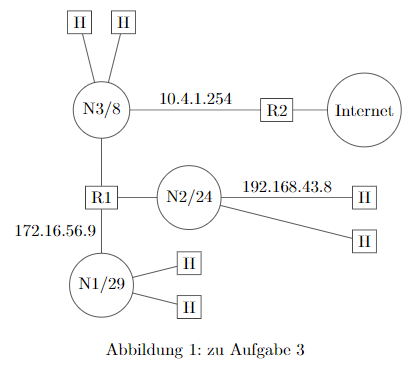
\includegraphics[scale=0.5]{bild1.png}
\end{center}


\textbf{Gesucht:}

a. Mögliche IP Adressen der Hosts/Repeater

b. Routingtabelle R1

c. ost im Netz N2 kann anderen Host im N2 erreichen, und Hosts im N1. Aber keineanderen Hosts d.h. auch nicht das Internet. Was wurde falsch konfiguriert?

\noindent 4.

\textbf{a.} Tabelle ausfüllen:

\newcommand{\tabincell}[2]{\begin{tabular}{@{}#1@{}}#2\end{tabular}}

\begin{tabular}{|c|c|c|c|c|}
    \hline
    Name der Schicht & Grundlegende Aufgabe & Transmission Unit & Adresse & Protokoll(Beispiel)\\
    \hline
    &&&Segment&\\
    \hline
    &&IP Adresse&&\\
    \hline
    &&&&HTTP\\
    \hline
    &\tabincell{c}{Erkennen von Über-\\ tragungsfehlern}&&&\\
    \hline
\end{tabular}
\\

\textbf{b.} Warum benötigt man IP Adressen, statt nur MAC Adressen?

\textbf{c.} Mit welchem Protokoll wird eine IP Adresse zu einer MAC Adresse aufgelöst?

\noindent 5.

\textbf{a.} Was wird übertragen wenn 111 mit CRC gesichert geschickt wird? (Generatorpolynom: $x^3+x^2+1$)?

\textbf{b.} Es wird ein Zyklischer Code mit den Elementen 01100, 00011 und 01111 betrachtet.Gehören 00110, 11110, 00000, 10000 zu diesem Zyklischen Code? Begründung!

\subsection{6}

\noindent \qquad \textbf{a.} Was bedeutet Zeile 4<img source=”/bla/blub.png” />

\noindent\qquad \textbf{b.} Wie lautet die erste Zeile des HTTP 1.1 Requests bei der Eingabe von ”miau” im Textfeldund der betätigung des submit Buttens?

\noindent\qquad \textbf{c.} Welche weitere Zeile ist mindestens noch in diesem HTTP 1.1 Request Enthalten?

\noindent\qquad \textbf{d.} Geben sie die Erste Zeile des HTTP Responses an.

\section{Ans 2016}

\noindent\textbf{A1}

(a)10111, g(x)=x3+x+1,求c(x)

(b)Die folgenden Codewöter sind Elemente eines Zyklischen Codes: 11000, 00011, 11110. Sind die Wörter 00111, 11011, 00000, 10000 ebenfalls Elemente dieses Codes?

\textbf{Ans:} (a) 略 (b) 循环码是线性码的子集,因此循环码可以使用线性码的性质:
两个输入该码的码字的和仍然属于该码的码字。
全零字总是一个码字。
一个线性码的两个码字之间的最小距离等于任何非零码字的最小汉明重量。
(循环码)不论循环位移多少次许用码,仍为许用码。那么$11000\oplus00011=11011\checkmark,00000\checkmark.\,10000\, und\, 00111\times $
\\
\noindent\textbf{A3} Was ist der Zweck der Port-Numern der Transportschicht?传输层端口号的目的是什么?

\textbf{Ans:} TCP und UDP der Transportschicht können Datenströme von mehreren Anwendungen empfangen, mit Portnummern identifizieren und dann zur Verarbeitung an die Internetschicht senden.
Gleichzeitig empfangen TCP und UDP Pakete von der Internetschicht, unterscheiden sie nach der Portnummer und geben sie dann an verschiedene Anwendungen weiter.

\noindent\textbf{A7} Ihr Rechner nutzt als Nameserver den von Ihrem Provider bereitgestellten Nameserver $resolv.provider.org$ mit der IP 9.9.9.9

(a)woher weiß ihr Rechner, welchen Nameserver er verwenden muss? 您的计算机如何知道使用哪个名称服务器?

(b)Geben Sie den FQDN für den Host mango an, welder sich in der Sub-Domäne informatik innerhalb der Domäne tu-chemnitz.de befindet.输入主机mango的FQDN,该mango位于域tu-chemnitz.de中的子域informatik中。

提示:FQDN(Fully Qualified Domain Name)全限定域名:同时代有主机名和域名的名称(通过符号”.”)。例如:主机名是bigserver,域名是mycompany.com,那么FQDN就是bigserver.mycompany.com。FQDN可以从逻辑上准确地表示出主机在什么地方,也可以说全域名是主机名的一种完全表示形式。

DNS解析流程:首先查找本机HOSTS表,有的直接使用表中定义,没有则查找网络连接中设置的DNS服务器由他来解析。

电子邮件地址就是典型的FQDN,@后面是邮件服务器的全域名,最后时顶层域名.com。FQDN=Hostname+DomainName

Nameserver: Ein Nameserver ist ein Server, der Namensauflösung anbietet. Namensauflösung ist das Verfahren, das es ermöglicht, Namen von Rechnern bzw. Diensten in eine vom Computer bearbeitbare Adresse aufzulösen.

\textbf{Ans:} (a) DNS kann URLs in IP-Adressen übersetzen. Der Domänenname besteht aus einer Folge von Wörtern oder Abkürzungen, die durch Punkte getrennt sind. Jeder Domänenname entspricht einer eindeutigen IP-Adresse. Es besteht eine Eins-zu-Eins-Entsprechung zwischen dem Domänennamen und der IP-Adresse im Internet. DNS ist der Server für die Auflösung von Domänennamen.

(b) mango.informatik.tu-chemnitz.de


\section{Ans 2015}

\textbf{A1} 

\qquad (a) Stellen Sie fest, ob die Bitfolgen 1010001 und 1100111 zum Code gehören! 确定位串1010001和1100111是否属于代码!

\qquad (b) Die Bitfolge 1001101 ist ein Codewort. Dekodieren Sie es!比特序列1001101是码字。解码它!


\qquad Ans:(a) Prüfungsmatrix= 
$\begin{pmatrix}
    1&1&1&0&1&0&0\\
    1&0&1&1&0&1&0\\
    0&1&1&1&0&0&1
\end{pmatrix}
$,
$P\cdot \begin{pmatrix}
    1\\0\\1\\0\\0\\0\\1
\end{pmatrix}$=000$\checkmark$,$P\cdot\begin{pmatrix}
    1\\1\\0\\0\\1\\1\\1
\end{pmatrix}$=100$\times$

\qquad Ans:(b) $P\cdot\begin{pmatrix}
    1\\0\\0\\1\\1\\0\\1
\end{pmatrix}$=000$\checkmark$ $\Rightarrow$Information: 1001

\noindent\textbf{A2} Was wird gesendet, wenn die Zeichenfolge 10111 durch einen zyklischen Code mit Generatorpolynom $g(x)=x^3+x+1$ geschützt wird? 当字符串10111受到具有生成多项式$g(x)=x^3+x+1$的循环码的保护时发送的是什么?

\quad Ans:

\qquad $g(x)\Rightarrow1011, r=3,p(x)=x^4+x^2+x+1\Rightarrow10111$

\qquad $CRC:p(x)\cdot x^r MOD g(x) = 10111000 \% 1011 = 011 $

\qquad $c(x) = 10111000\oplus 011 = 10111011$

\noindent\textbf{A3} Schreiben Sie in Python einen Server, der auf TCP-Port 8080 läuft und an ihn gesendete Wörter erwartet. Als Rückgabe sendet er eine Zahl, die angibt, wie oft dieses Wort seit dem Server-Start bereits an ihn gesendet wurde. 在Python中,编写一个在TCP端口8080上运行的服务器,并期望将字发送给它。 作为回报,他发送一个数字,表示自服务器启动以来该字被发送给他的次数。

Die folgende Telnet-Sitzung soll das Verhalten des Server verdeutlichen: 以下Telnet会话应阐明服务器的行为:

\fbox{\shortstack[l]{
\$ telnet alpha.local.de 8080\\
World\\
1\\
Connection closed by foreign host.\\
\\
\$ telnet alpha.local.de 8080\\
Live\\
1\\
Connection closed by foreign host.\\
\\
\$ telnet alpha.local.de 8080\\
Live\\
2\\
Connection closed by foreign host.
}
}
\fbox{\shortstack[l]{
\$ telnet alpha.local.de 8080\\
Live\\
3\\
Connection closed by foreign host.\\
\\
\$ telnet alpha.local.de 8080\\
World\\
2\\
Connection closed by foreign host.\\
\\
\$ telnet alpha.local.de 8080\\
ooo\\
1\\
Connection closed by foreign host.
}
}

提示1:Nehmen Sie folgende Funktion zum Lesen erner Zeile vom Socket als gegeben an (nicht abschreiben)假设以下函数用于从给定的套接字读取一行(不要直接抄):
\begin{lstlisting}
def recvline(conn):
    data = ''
    while 1:
        d=conn.recv(1)
        if d == ‘\n’:
            break
        if d !=’\r’:
            data = data + d
        return data
\end{lstlisting}

提示2:Flüchtigkeitsfehler, die beim ersten Programmlauf schnell gefunden würden, bleiben bei der Korrektur unberücksichtigt.在校正中不考虑在第一次运行时快速发现的滑移误差。

提示3:Auf Plausibilitäts- und Eingabefehlerkontrollen kann komplett verzichtet werden.关于合理性和输入错误检查可以完全省略。

提示4:可能有用的:
str (3) aus dem Zahlenwert 3 den StringWert '3' erzeugt. str(3)从数字3生成字符串值'3'。
dict.has-key('ff')仅当字典中含有键('ff')时为真。

Ans:

\begin{lstlisting}
#Server
import socket
PORT=8080
s=socket.socket(socket.AF_INET,socket.SOCK_STREAM)
s.bind(("localhost",PORT))
s.listen(1)
data=[]
count=[]
def count_num(from_c):
    index = 0
    for i in range(len(data)):
        if data[i]==from_c:
            index = i
    if from_c not in data:
        data.append(from_c)
        count.append(1)
        return "1"
    else:
        count[index] = count[index] + 1
        return str(count[index])
while True:
    conn,addr = s.accept()
    msg = conn.recv(1024)
    sendmsg = count_num(msg.decode())
    conn.send(sendmsg.encode())
    conn.close()
s.close()
\end{lstlisting}

\noindent\textbf{A4} Warum gibt es beim TCP einen 3 - WegeHandshake?为什么TCP上有3次握手?
提示:仅回答“连接”是不够的。重点是3!如果两个合作伙伴同意相互联系,则两个合作伙伴中的每一个都同意这样做就足够了,即交换了两条消息。但是使用TCP有3条消息。为什么呢?

\textbf{Ans:}Drei Handshakes sind erforderlich, um zu bestätigen, ob die Empfangs- und Sendefunktionen beider Parteien normal sind.
需要三次握手才能确认双方的接收与发送能力是否正常。

为什么2次不行?答:可能的情况如客户端发出连接请求,但因连接请求报文丢失而未收到确认,于是客户端再重传一次连接请求。后来收到了确认,建立了连接。数据传输完毕后,就释放了连接,客户端共发出了两个连接请求报文段,其中第一个丢失,第二个到达了服务端
Wenn der Client eine Verbindungsanforderung sendet, das Verbindungsanforderungspaket jedoch verloren geht und keine Bestätigung empfangen wird, überträgt der Client die Verbindungsanforderung erneut. Später erhielt es eine Bestätigung und stellte eine Verbindung her. Nach Abschluss der Datenübertragung wird die Verbindung freigegeben. Der Client sendet insgesamt zwei Verbindungsanforderungssegmente, von denen das erste verloren geht und das zweite den Server erreicht.

为什么关闭连接是4次握手?答:关闭连接时,当收到对方的FIN报文通知时,它仅仅表示对方没有数据发送给你了;但未必你所有的数据都全部发送给对方了,所以你可能未必会马上会关闭SOCKET,也即你可能还需要发送一些数据给对方之后,再发送FIN报文给对方来表示你同意现在可以关闭连接了,所以它这里的ACK报文和FIN报文多数情况下都是分开发送的。
Wenn Sie die Verbindung schließen und die FIN-Nachrichtenbenachrichtigung der anderen Partei erhalten, bedeutet dies nur, dass die andere Partei keine Daten zum Senden an Sie hat, aber nicht alle Ihre Daten an die andere Partei gesendet wurden, sodass Sie SOCKET möglicherweise auch nicht sofort schließen Das heißt, Sie müssen möglicherweise einige Daten an die andere Partei senden und dann eine FIN-Nachricht an die andere Partei senden, um anzuzeigen, dass Sie damit einverstanden sind, die Verbindung jetzt zu schließen. Daher werden die meisten ACK-Nachrichten und FIN-Nachrichten hier separat gesendet.

\noindent\textbf{A5} Wieso ist die digitale Übertragung (auch ohne Prüfsummenbildung !!!) weniger Störanfällig als die analoge Übertragung?为什么数字传输(即使没有校验和形成!!!)比模拟传输更不容易受到干扰?

\textbf{Ans:}Das analoge Signal hat keine Lösung für alle Arten von Interferenzen und kann nur beim Empfang ausprobiert werden.
Bei digitalen Signalen können diese Störungen jedoch durch spezielle Codierungs- und Demodulationsverfahren während der Übertragung behandelt werden.
z.B. Fehlerkorrekturcode-Technologie.

模拟信号无法解决所有类型的干扰,只能在收到模拟信号后才能试用。
但是,在数字信号的情况下,可以在传输期间通过特殊的编码和解调方法来处理这些干扰。
例如 纠错码技术。

\noindent\textbf{A6} Wie viel Bit können bei einer 128 QAM in einem Schritt übertragen werden?用128 QAM一次可以传输多少Bit?

\textbf{Ans:}  log128 = 7 bit

\noindent\textbf{A7} Unter http://www.venturel.com ist folgende WEB-Seite erreichbar:在该网址上可以找到以下WEB页面:

\begin{lstlisting}
<html>
    <head><title>LIST</title></head>
    <body>
        <h1>List</h1><hr/>
        <p><a href="/left">side-by-side</a></p> 
        <p><a href="/rotated">turned</a></p> 
        <p><a href="/standing">fixed</a></p> 
        <p><a href="/falling">insecure</a></p> 
        <p><a href="/cutted">knife</a></p>
    </body>
</html>
\end{lstlisting}

(a)Wie lautet die erste Zeile des HTTP-1.1-GET-Requests, wenn der Nutzer auf den Link mit der Beschriftung "fixed" klickt?当用户点击标记为“已修复”的链接时,HTTP 1.1 GET请求的第一行是什么?

(b)Welche weitere Zeile ist in diesem HTTP-1.1-GET-Requests wenigstens noch enthalten?哪个附加行至少仍包含在此HTTP 1.1 GET请求中?

(c)Welchen Sinn hat diese weitere Zeile?何种意义上这进一步行?

\textbf{Ans:} (a) GET / HTTP/1.1 \qquad (b) Host: www.venturel.com \qquad (c) Ein HTTP-1.1-Proxy muss sicherstellen, dass jede von ihm weitergeleitete Anforderungsnachricht ein geeignetes Host-Header-Feld enthält, das den vom Proxy angeforderten Dienst identifiziert.

\noindent\textbf{A8}有以下网络图

\begin{center}
    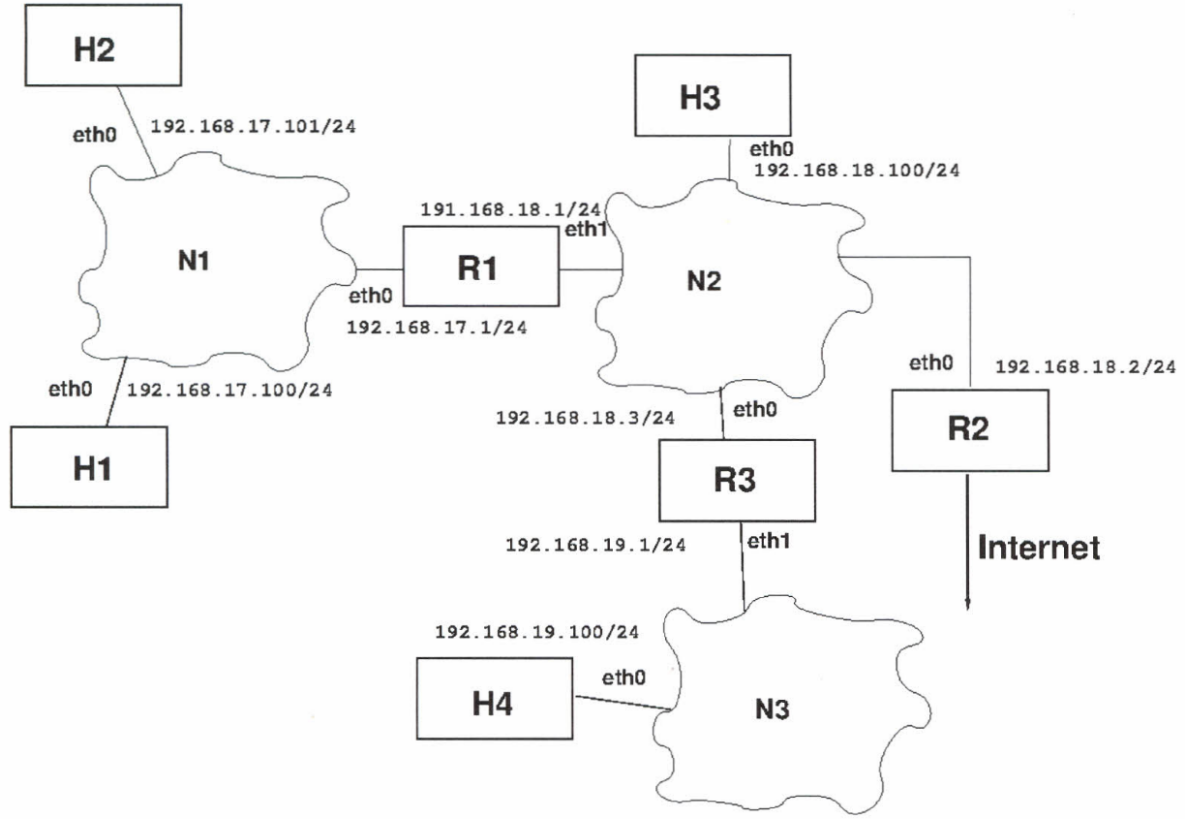
\includegraphics[]{bild2.png}
\end{center}

Die Router R1, R2 und R3 verbinden die Subnetze N1, N2und N3miteinander. Der Router R2 hat außerdem einen Zugang zum Internet. 
Dort stellt der Service-Provider den (nicht dargestellten) Router 1. 2 . 3 . 4 ins Internet zur Verfügung.
Die Hosts Hl und H2 sind ans Netz N1 angeschlossen. Der Host H3ist ans Netz N2 und der Host H4 ist ans Netz N3 angeschlossen.

路由器R1,R2和R3将子网N1,N2和N3彼此连接。路由器R2还可以访问Internet。
在那里,服务提供商(未示出)路由器1。第三 4可在互联网上找到。
主机H1和H2连接到网络N1。主机H3连接到网络N2,主机H4连接到网络N3。

(a)Schreiben Sie die Routingtabelle für den Router R1! 写出R1的路由表

提示1:Die Tabelle muss die Kommunikation mit allen gezeigten Netzknoten (Routern, Hosts) sowie zum Internet ermöglichen.该表必须能够与所有显示的网络节点(路由器,主机)以及Internet进行通信。

提示2:Host-spezifische Routen sind nicht erlaubt.不允许特定于主机的路由。

\textbf{Ans:}

\begin{tabular}{|c|c|c|c|}
    \hline
    Ziel&Netzmaske&Gateway&Interface\\
    \hline
    192.168.17.0&255.255.255.0(/24)&*&Eth0\\
    \hline
    192.168.18.0&/24&*&Eth1\\
    \hline
    192.168.19.0&/24&192.168.18.3&Eth1\\
    \hline
    Default&0.0.0.0&192.168.18.2&Eth1\\
    \hline
\end{tabular}

\section{Ans 2014}

\noindent\textbf{A1} (a)Was wird übertragen, wenn die Bitfolge 10001 durch einen zyklischen Code mit dem Generatorpolynom $g(x) = x^3 + x + 1$ geschützt wird?如果比特序列10001受到具有生成多项式$g(x) = x^3 + x + 1$的循环码的保护,则发送什么?

(b)Rechnen Sie vor, wie der Empfänger die Richtigkeit testet! Woran erkennt der Empfänger die Richtigkeit der Bitfolge?计算接收器如何测试正确性!接收器如何识别位序列的正确性?

\textbf{Ans:}$p(x)=x^4+1\Rightarrow10001,r=3,CRC:(x^7+x^3)\%g(x)\Rightarrow10001000:1011=10$

$c(x)=10001010$

$Probe:10001010:1011=0$

\noindent\textbf{A2} 有以下网络:

\begin{center}
    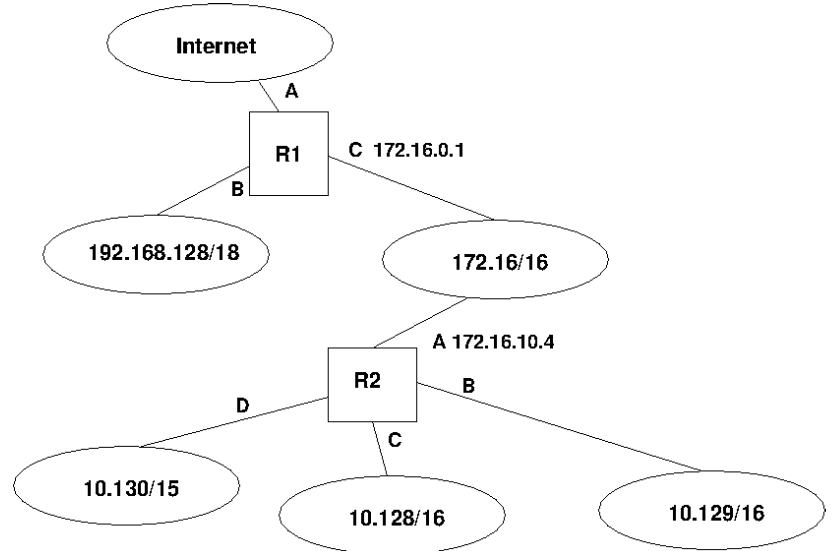
\includegraphics[scale=0.5]{bild3.png}
\end{center}

Die Router R1 und R2 sollen konfiguriert werden. Schreiben Sie die Routing­Tabelle für die beiden Router! Der Service­Provider stellt den (nicht dargestellten) Router 1.2.3.4 ins Internet zur Verfügung.

要配置路由器R1和R2。 写两个路由器的路由表! 服务提供商使因特网上的路由器1.2.3.4(未示出)可用。

\textbf{Ans:} (考试时不要用ABC简写)

\begin{tabular}{|c|c|c|c|}
    \hline
    Ziel&Netzmaske&Gateway&Interface\\
    \hline
    R1\\
    \hline
    Internet/default&0.0.0.0&*&A\\
    \hline
    192.168.128.0&255.255.192.0&*&B\\
    \hline
    172.16.0.0&255.255.0.0&*&C\\
    \hline
    10.130.0.0&255.254.0.0&A&C\\
    \hline
    10.128.0.0&255.255.0.0&A&C\\
    \hline
    10.129.0.0&255.255.0.0&A&C\\
    \hline
\end{tabular}

\noindent\textbf{A3} Sie wollen auf die Seite http://www.mysql.com zugreifen. Sie erhalten eine Fehlernachricht, dass dies nicht möglich ist.
您想要访问页面http://www.mysql.com。您收到一条错误消息,指出“这是不可能的”。

Nennen Sie in jeder Schicht des Internet­Protokollstacks je eine mögliche Fehlerursache!在Internet协议栈的每一层中列出一个可能的失败原因!

\begin{tabular}{c|c}
    L1&Kabel bruch\\
    L2&Kollisionen von Package\\
    L3&Routing-Tabelle (fehlerhafte)\\
    L4&Firewall verbietet Ports\\
    L5-L7&Browser-Programmfehler 
\end{tabular}

\noindent\textbf{A5} (a)Schreiben Sie eine WEB­Seite, die aus Nutzersicht folgendes Aussehen hat:从用户的角度编写具有以下外观的WEB页面:(左图)


\includegraphics[]{bild4.png}\qquad
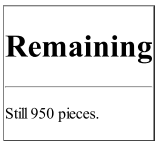
\includegraphics[]{bild5.png}

Die Phrasen "\,One piece", "\,Five pieces\,"\, und "\,Ten pieces"\, sollen Hypertext­Links sein!短语“One piece”,“Five pieces”和“Ten pieces”应该是超链接!

(b) Schreiben Sie einen zugehörigen TCP­Server in Python, sodass jeder Klick auf "\,One piece", "\,Five pieces\,"\, oder "\,Ten pieces"\, auf (etwa) folgende WEB­Seite führt:在Python中编写一个关联的TCPServer,以便每次单击“One piece”,“Five pieces”或“Ten pieces”导致(大约)以下WEBSite:(右图)

\textbf{Ans:}

\textbf{(a)}

\begin{lstlisting}
<!--index.html-->
<html>
<head>
    <link rel="stylesheet" type="text/css" href="index.css">
    <meta charset="UTF-8">
</head>
<body>
    <table class="abc">
        <tr>
            <td>Shop<HR></td>
        </tr>
        <tr>
            <td action="http://localhost:8080">
                <a href="http://localhost:8080/one">One piece</a><br/>
                <a href="http://localhost:8080/one">Five piece</a><br/>
                <a href="http://localhost:8080/one">Ten piece</a>
            </td>
        </tr>
    </table>
    <table class="abc">
        <tr>
            <td>Remaining<hr></td>
        </tr>
        <tr>
            <td>Still 1000 pieces.</td>
        </tr>
    </table>
</body>
</html>
\end{lstlisting}

\begin{lstlisting}
/*index.css*/
table.abc{
    border : 2px solid black;
    border-style:solid;
    
    padding:0;
    margin:10;
}
\end{lstlisting}

\textbf{(b)}

\begin{lstlisting}
import socket

s = socket.socket(socket.AF_INET,socket.SOCK_STREAM)
s.bind(("",8080))
s.listen(1)
print("Server started")
stock = 1000

while True:
    conn, addr = s.accept()
    msg = conn.recv(1024)
    userRequest = msg.decode().split()
    if userRequest[1] == "/one":
        stock -= 1
    elif userRequest[1] == "/five":
        stock -= 5
    elif userRequest[1] == "/ten":
        stock -= 10
    answer = """HTTP/1.1 200 OK\n\n<html>
<head>
    <style media="screen" type="text/css">
        table.abc {
            border: 2px solid black;
            border-style: solid;
            padding: 0;
            margin: 10;
}
    </style>
    <meta charset="UTF-8">
</head>
<body>
    <table class="abc">
        <tr>
            <td>Shop<HR></td>
        </tr>
        <tr>
            <td action="http://localhost:8080">
                <a href="http://localhost:8080/one">One piece</a><br />
                <a href="http://localhost:8080/five">Five piece</a><br />
                <a href="http://localhost:8080/ten">Ten piece</a>
            </td>
        </tr>
    </table>
    <table class="abc">
        <tr>
            <td>Remaining<hr></td>
        </tr>
        <tr>
            <td>Still"""+str(stock)+"""pieces.</td>
        </tr>
    </table>
</body>
</html>
"""
    conn.send(answer.encode())
    conn.close()
s.close()
\end{lstlisting}

\section{Ans 2012}

\noindent\textbf{A1} Die folgenden Bitfolgen sind Elemente des linearen Codes C1. 以下位串是线性代码C1的元素:$\cdot10100011 $ \qquad $\cdot 01101001$

(a)Ist 11001010 auch Element des linearen Codes C1. 也是线性代码C1的元素吗?

(b)论证

\textbf{Ans:}(a)$10100011 \oplus01101001 = 11001010\checkmark$ (b) Summer zweier gültiger Codeworte ist ebenfalls ein gültiges Codewort (Modulo-Arithmetik).

\noindent\textbf{A3} Ethernet-Adressen sind weltweit eindeutig! Warum benutzt man diese nicht gleich als IPAdressen?
Hinweis: Die Antwort lautet nicht: "Weil nicht jeder Host über Ethernet ans Internet angeschlossen ist.". Das ist zwar wahr, aber selbst wenn dem so wäre, ginge es nicht.
以太网地址在全球范围内独 为什么不立即将它们用作IP地址?
注意:答案不是,“因为不是每个主机都通过以太网连接到Internet。”这是真的,但即使它是,它也行不通。

\textbf{Ans:}

(1) IP兼容性强,物理层技术不仅有Ethernet. Die IP-Kompatibilität ist stark und die Technologie der physischen Schicht besteht nicht nur aus Ethernet.

(2) IP简单化了Internet转发规则。IP vereinfacht die Regeln für die Internetweiterleitung.

(3) 路由器不可能记住所有MAC地址。但通过IP地址的前缀就可以知道设备在哪个子网上了,减少了路由器所需要的内存。Der Router kann sich nicht alle MAC-Adressen merken. Durch das Präfix der IP-Adresse können Sie jedoch erkennen, in welchem ​​Subnetz sich das Gerät befindet, wodurch der vom Router benötigte Speicher reduziert wird.

\textbf{课件中:}

\textit{(1)Ethernet skaliert nich auf globales Level. (Broadcasts, Switches, Anzahl Hubs, Signallaufzeiten)\\\indent (2)Nicht alle Netze nutzen die selbe Subnetz-Technologie (technische Gründe)\\\indent (3)Gemeinsamer, effizienter "Nenner" für gesamtes Netz notwendig}

\noindent\textbf{A4} 

(a) Nennen Sie ein Szenario, wo NAT (Network Address Translation) eingesetzt wird!请给出一个使用NAT的场景。

(b) Eine Schule ist per NAT ans Internet angebunden. 学校通过NAT连接到互联网:

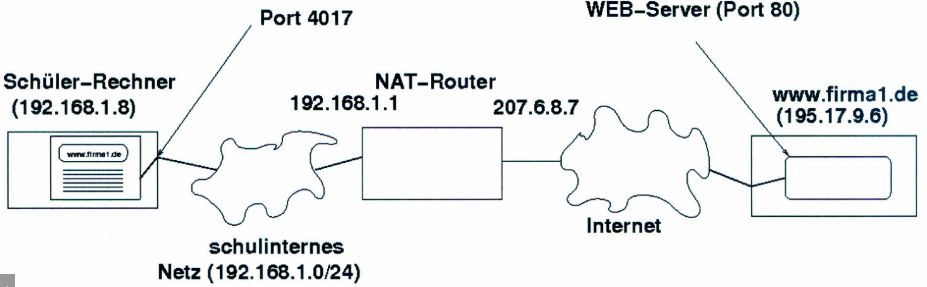
\includegraphics[scale = 0.6]{bild6.png}

Der NAT-Router habe die IP-Adresse 192.168.1.1 zum internen Schulnetz hin. Bei der Anmeldung am Internet ist ihm die IP-Adresse 207.6.8.7 zugewiesen worden.NAT路由器具有朝向内部学校网络的IP地址192.168.1.1。 登录到Internet时,已为其分配IP地址207.6.8.7。

Ein Schüler am Rechner mit der IP-Adresse 192.168.1.8 tippt in seinen WEB-Browser den URL: 在他的WEB浏览器中,IP地址为192.168.1.8的计算机上的学生URL:

$http://www.firma1.de/ $

\noindent ein. Der Rechner www.firma1. de habe die IP-Adresse: 195.17.9.6.

Welchen Eintrag nimmt daraufhin der NAT-Router in seiner NAT-Tabelle vor, wenn ferner angenommen wird, dass sich der WEB-Browser zum Aufbau der vom Schüler angewiesenen Kommunikation auf Port 4017 gebunden hat? Wählen Sie weitere dazu benötigte Nummern und/oder Adressen selbst!

如果假设WEB浏览器已经绑定自己在端口4017上建立学生指导的通信,那么NAT路由器在其NAT表中做了什么条目?自己选择所需的其他数字和/或地址!

(c)Was wird bei oben beschriebener Kommunikation bei der Vermittlung durch den NAT-Router gemäß Ihrer Lösung 4b im Request-Paket ausgetauscht?

Hinweis 1: Nennen Sie die konkreten Zahlen bzw. Werte! Welche Zahl bzw. welcher Wert wird durch welche Zahl bzw. Wert ersetzt?

Hinweis 2: Beschreiben Sie nur die wegen NAT getätigten Änderungen! Beschreiben Sie nicht das gesamte Paket oder komplette Header!

根据您的解决方案4b,NAT路由器在上述通信的请求包中交换了什么?

注1:命名具体的数字或值!哪个数字或哪个值被哪个数字或值替换?

注2:仅描述因NAT而发生的变化!不要描述整个包裹或完整标题!

\textbf{Ans:}

(a) Benutzer müssen auf das Internet zugreifen, der Host verfügt jedoch nicht über eine global eindeutige IP-Adresse.

(b) \begin{tabular}{|c|c|}
    \hline
    Inside Local IP Adresses & Inside Global IP Addresses\\
    \hline
    192.168.1.8:4017&207.6.8.7:4017\\
    \hline
\end{tabular}

(c) 192.168.1.8 $\rightarrow$ 207.6.8.7

\noindent\textbf{A5} 

(a) Zeichnen Sie den störungsfreien Verbindungsaufbau von TCP als WegZeitdiagramm auf!记录TCP的无故障连接设置作为路径时间图!

(b)Die Firewall eines Instituts soll durch geschicktes Löschen von TCP-Segmenten nur solche TCP- Verbindungen zulassen, die vom Inneren des Institutes zu einem Ziel außerhalb des Institutes aufgebaut werden. Welche TCP-Segmente muss die Firewall demzufolge löschen? Beschreiben Sie, woran genau die Firewall die zu löschenden TCPSegmente erkennt!

Hinweis 1: Die Antwort lautet nicht: "Die Firewall muss alle TCP-Segmente löschen, die von außerhalb des Institutes kommen!", denn auf jeden per TCP gesendeten Request, folgt natürlich ein Reply von außerhalb, der gleichfalls per TCP ankommt. Würde man alle von außerhalb eintreffenden TCP-Segmente löschen, so würde kein einziger Reply mehr das Institut erreichen, was im Effekt dem Kappen der Internetverbindung gleichkommt!

Hinweis 2: Es geht um alle TCP-Dienste (telnet, ssh, pop, imap, smtp, http, ftp, selbstgebastelte Dienste, z.B.: mit Python-Sockets, ...).

通过巧妙地删除TCP段,研究所的防火墙应该只允许从研究所内部建立的TCP连接到研究所外的目的地。防火墙必须删除哪些TCP段?描述防火墙究竟检测到要删除的TCPS段的确切内容!

注1:答案不是:“防火墙必须删除来自机构外部的所有TCP段!”,因为每个通过TCP发送的请求当然都是来自外部的回复,这也是通过TCP到达的。如果要从外部删除所有传入的TCP片段,那么不再有一个单一的答复会再到达该学院,这实际上等于互联网连接的上限!

注2:它是关于所有TCP服务的。

\textbf{Ans:}

(a) 
\begin{center}
    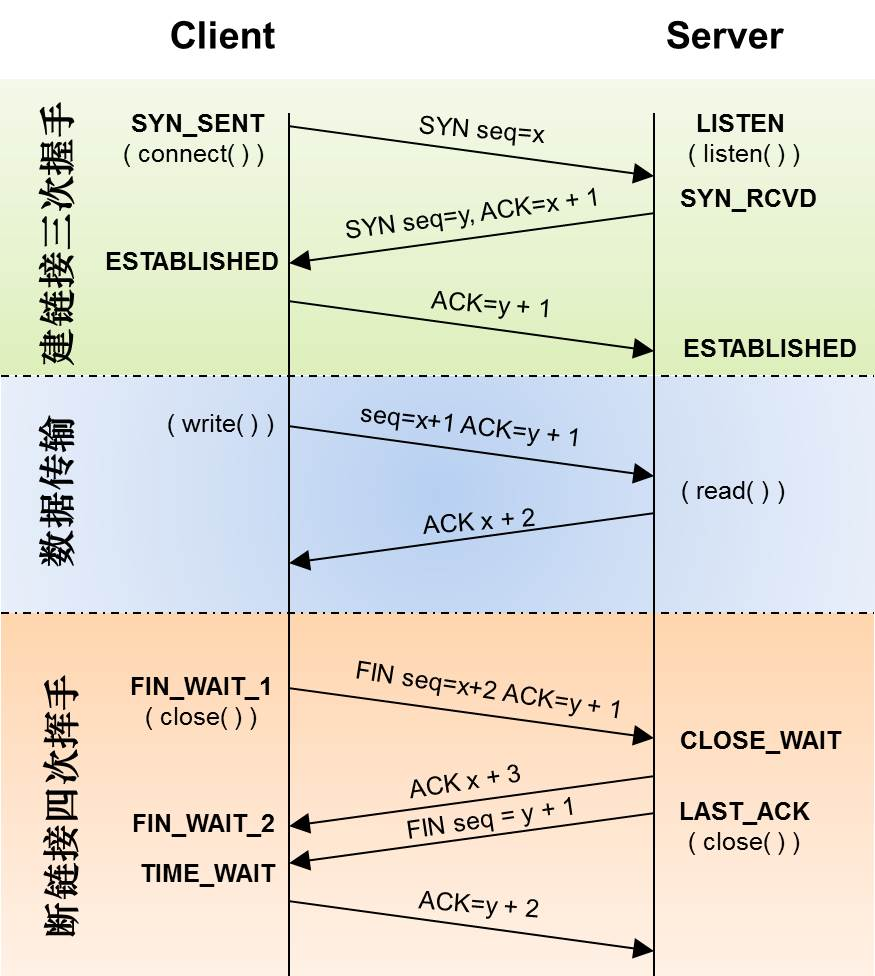
\includegraphics[scale=0.6]{bild7.jpg}
\end{center}

(b) 不知。

\noindent\textbf{A6} Schreiben Sie zwei Python-Programme, welche einen Server und einen zugehörigen Klienten bilden, und das entfernte Berechnen einfacher Aufgaben erlauben.
Da das Protokoll HTTP-konform sein soll, erwartet der Klient als Nutzereingabe einen URL folgenden Aufbaus:

编写两个构成服务器和关联客户端的Python程序,允许远程计算简单任务。
由于协议是HTTP兼容的,因此客户端需要以下结构的用户输入URL:

$http://<Rechnername>:<port>/<operation>/<operand1 >/<operand2 >$

其中:

<Rechnername> ein beliebiger Rechnername. Es wird angenommen, dass der von Ihnen geschriebene Server dort gestartet wurde.

<port> ein beliebiger Port. Es wird angenommen, dass sich der von Ihnen geschriebene Server sich auf diesen Port gebunden hat.

<operation> entweder add oder sub oder mul. Der Server soll gemäß dieser Angabe die beiden Operanden entweder addieren oder subtrahieren oder multiplizieren. • <operand1>, <operand2> beliebige ganze Zahlen.

<Rechnername>任何计算机名称。假设您编写的服务器是在那里启动的。

<port>任何端口。假设您编写的服务器绑定到此端口。

<operation> add或sub或mul。服务器应根据此规范添加或减去或乘以两个操作数。 •<operand1>,<operand2>任意整数。

示例输入:$http://mein.grosser .rechner. de: 7829/add/12/3 \Rightarrow 15$

Hinweis 1: Beachten Sie bitte, dass das Protokoll zwischen Client und Server HTTP sein soll!请注意客户端和服务器之间的协议应该是HTTP!

Hinweis 2: Nehmen Sie die Funktion recv line zum Lesen einer Zeile von einem Socket als gegeben an (nicht abschreiben!!!)考虑函数recv行从给定的套接字读取一行(不要抄写!!!)
此处代码段与SS2015-A3和WS2014-A5b相同

Hinweis 3: Das Ergebnis muss nicht aufbereitet werden, sondern kann so, wie es der Client vom Server empfangt auf der Konsole ausgegeben werden.

Hinweis 4: Flüchtigkeitsfehler, die bei einem ersten Testlauf des Programms schnell gefunden würden, bleiben bei der Korrektur unberücksichtigt.

Hinweis 5: Auf das Prüfen der Nutzereingaben (Plausibilitätskontrollen) kann komplett verzichtet werden.

Hinweis 6: Der Server-Port soll als Argument an den Server übergeben werden.

注3:结果不需要呈现,但可以在客户端从服务器接收时输出到控制台。

注4:在校正过程中不考虑在程序的第一次测试运行中快速发现的跳过错误。

注5:可以完全省去检查用户输入(合理性检查)。

注6:服务器端口应作为参数传递给服务器。

Hinweis 7: Möglicherweise ist es hilfreich zu wissen, dass eine Zeichenkette eine Methode split () anbietet, die die Zeichenkette an Leerzeichen splittet und eine Liste mit dem Ergebnis zurückgibt: s = "aaa bbb" s.splin) --> ['aaa', 'bbb']
Gibt man ein Argument an, so wird dieses Symbol als Trennzeichen betrachtet: s="solokoffer" s.split('o') --> ['s', '1', 'k', 'ffer']

注7:知道字符串提供split()方法可能会有所帮助,该方法分割空格字符串并返回结果列表:s =“aaa bbb”s.splin) - > ['aaa ','bbb']
如果你指定一个参数,这个符号将被视为一个分隔符:s =“solobox”s.split('o') - > ['s','1','k','ffer']

\begin{lstlisting}
#Server
import socket
PORT=8080
s=socket.socket(socket.AF_INET,socket.SOCK_STREAM)
s.bind(("localhost",PORT))
s.listen(1)
op = ["add","sub","mul"]
def count_num(from_c):
    data = from_c.split('/')
    data = data[-3:]
    if data[0]==op[0]:
        return str(int(data[1])+int(data[2]))
    if data[0]==op[1]:
        return str(int(data[1])-int(data[2]))
    if data[0]==op[2]:
        return str(int(data[1])*int(data[2]))
    return "false"
while True:
    conn,addr = s.accept()
    msg = conn.recv(1024)
    sendmsg = count_num(msg.decode())
    conn.send(sendmsg.encode())
    conn.close()
s.close()
\end{lstlisting}

\section{Ans 09}

\noindent 网页邮件

Sie kennen sicherlich sogenannte Web-Mailer, also WWW-Oberflächen über die Sie E-Mails lesen und vielleicht sogar schreiben können. Ihre Aufgabe ist es nun, einen einfachen Web-Mailer zu schreiben.

Zum Ausprobieren steht ein Test-POP-Server zur Verfügung 

\qquad Rechner taurus.informatik.tu-chemnitz.de, Port 110 

\qquad Nutzer rot und Passwort rot

Hinweise: 

\qquad Vorab Eingabe von POP-Server, Benutzername, Passwort

\qquad Design der Webseiten ist nicht relevant 

\qquad es reicht, wenn man E-Mails lesen kann

\textbf{mail.py}
\begin{lstlisting}
import socket,poplib,email,sys
PORT=8080
s = socket.socket(socket.AF_INET,socket.SOCK_STREAM)
s.bind(("",PORT))
s.listen(1)
pop3_server = "taurus.informatik.tu-chemnitz.de"
#上面有效部分为建立与localhost:8080的通道
conn, addr = s.accept()
#从网页(localhost:8080)接收数据,对数据进行记录
def recvline(conn):
    data=''
    while 1:
        d = conn.recv(1024)
        if d == '\n':
            break
        if d!='\r':
            data = data + d.decode()
        #print(data)
        #conn.close()
        return data
#(尝试,不一定能成功)将邮件信息打印出来,函数在HTML中间被调用
def printmail(mailbox):
    for i in range(len(mailbox)):
        print("The "+i+" Mail")
        for j in range(len(mailbox[i])):
            print(mailbox[i][j])     
#获取邮件
def getmail(server):
    ret = server.stat()
    rsp,msg,siz= server.retr(server.stat()[0])
    index = len(server.list()[1])
    mailbox = []
    for i in range(index):
        lines = server.retr(i+1)[1]
        msg_content = b'\r\n'.join(lines).decode('utf-8')
        mailbox.append([])
        tmsg = msg_content.split('\n')
        mailbox[i].append(tmsg)
    return mailbox
#从网页(login.html)获取用户名和密码,并记录
l = recvline(conn)
user = l.split('\n')[-1:]
user = (str(user[0])).split('&')
userName = user[0][-3:]
userPassword = user[1][-3:]
#建立于学校内网的连接
server = poplib.POP3(pop3_server)
#(不知道返回值是啥,因此不确定此处是否能正常运行)判断用户名和密码是否正确,若正确,则继续
if server.user(userName) and server.pass_(userPassword):
    while 1:
        conn, addr = s.accept()
        msg = conn.recv(1024)
        userRequest = msg.decode().split()
        if userRequest[1] == "/aktuallisieren":
            getmail(server)
        if userRequest[1] == "/serverbeenden":
            conn.close()
            server.quit()
            answer = """HTTP/1.1 200 OK\n\n<html>
<head>
    <meta charset="UTF-8">
</head>
<body>
<h1>abgemeldet!</h1>
</body>
"""
        answer = """HTTP/1.1 200 OK\n\n<html>
<head>
    <meta charset="UTF-8">
</head>
<body>
    <table>
        <tr>
            <td>Webmailer Uebersicht</td>
        </tr>
        <tr>
          <td action="http://localhost:8080">
            <a href="http://localhost:8080/aktuallisieren">aktuallisieren</a><br />
            <a href="http://localhost:8080/serverbeenden">Server beenden</a><br />
          </td>
        </tr>
        <tr>
            <td action="http://localhost:8080">
                """+ printmail(getmail(server)) +"""
            </td>
        </tr>
    </table>
</body>
</html>"""
        conn.send(answer.encode())
    conn.close()
server.quit()
s.close()
\end{lstlisting}

\textbf{login.html}
\begin{lstlisting}
<html>
  <head>
    <title></title>
    <meta content="UTF-8">
    <style></style>
  </head>
  <body>
    <form method="POST" action="http://localhost:8080">
      Benutzername:<input type="text" name="username"/><br/>
      Passwort:<input type="password" name="passwprd"/><br/>
      <input type="submit" value="Anmelden"/>
    </form>
  </body>
</html>
\end{lstlisting}

\textbf{mail.html}
\begin{lstlisting}
<html>
<head>
    <meta charset="UTF-8">
</head>
<body>
    <table>
        <tr>
            <td>Webmailer Uebersicht</td>
        </tr>
        <tr>
          <td action="http://localhost:8080">
            <a href="http://localhost:8080/aktuallisieren">aktuallisieren</a><br />
            <a href="http://localhost:8080/serverbeenden">Server beenden</a><br />
          </td>
        </tr>
    </table>
</body>
</html>
\end{lstlisting}



\section{Ans 05}

\noindent Implementieren Sie eine einfache Switching Engine. 实现简单交换机

Der "Switch" besteht aus N Anschlüssen. “开关”由N个连接组成。

Zur Vereinfachung gibt es maximal 255 Adressen, wobei die Adresse 255 als Broadcast-Adresse verwendet wird.
为简化起见,最多有255个地址,地址255用作广播地址。

Es wird ein Paketkopf gelesen und entsprechend des Zustandes der Engine entschieden, auf welchen Anschluss das zugehörige Paket geschickt wird.
读取标头,并确定引擎的哪个状态到相应数据包的端口。

Informationen, die an die Engine geliefert werden, sind Eingangsportnummer (1..N), Absenderadresse (1..255) und Zieladresse (1..255).
提供给引擎的信息是输入端口号(1..N),发送方地址(1..255)和目标地址(1..255)。

Die Engine bestimmt daraufhin das Ziel und gibt diese Information aus.
然后引擎确定目的地并输出此信息。

Mit der Eingabe von "a" wird die Ausgabe der Adresstabellen ausgelöst.
输入“a”会触发地址表的输出。

6端口交换机的可能示例会话:

\fbox{
    \shortstack[l]{
switch< 1 23 54\\
switch> Ausgabe auf allen Ports\\
switch< 4 32 23 \\
switch> Ausgabe auf Port 1 \\
switch< 6 35 32 \\
switch> Ausgabe auf Port 4 \\ 
switch< 2 32 23 \\
switch> Ausgabe auf Port 1 \\
switch< 6 85 32 \\
switch> Ausgabe auf Port 2\\
switch< 1 55 35 \\
switch> Ausgabe auf Port 6 \\
switch< 6 5 255 \\
switch> Ausgabe auf allen Ports \\
switch< a \\
switch> 
    }
}
\fbox{\shortstack[l]{1: 23 55 \\
2: 32 \\
3: \\
4: \\
5: \\
6: 35 85 5}}

\textbf{Ans:}

\begin{lstlisting}
data = [int(x) for x in input('switch<').split()]
port =[[] for i in range(6)]
print(port)
def find(a,b):
    n = len(a)
    for i in range(0,n):
        m = len(a[i])
        for j in range(0,m):
            if b == a[i][j]:
                return i+1
    return -1
def aging(a,b,c):
    n = len(a)
    for i in range(0,n):
        m = len(a[i])
        for j in range(0,m):
            if b == a[i][j] and c != i:
                a[i].pop(j)
                return
while data[0] != 'a':
    print(data)
    (port[data[0]-1]).append(data[1])
    num = find(port,data[2])
    aging(port,data[1],data[0]-1)
    if num == -1:
        print("switch>Ausgabe auf allen Ports")
    else:
        print("switch>Ausgabe auf Port",end=" ")
        print(num)
    print(port)
    data = [int(x) for x in input('switch<').split()]
print("switch>")
n = len(port)
for i in range(0,n):
    print("i+1:",end=" ")
    m = len(port[i])
    for j in range(0,m):
        print(port[i][j],end="")
    print()
\end{lstlisting}

\clearpage

\section{概念题}

1. 网络协议主要要素为:语法、语义、同步

2. 一座大楼内的一个计算机网络系统,属于:LAN

3. 随着电信和信息技术的发展,国际上出现了所谓“三网融合”的趋势,下列属于三网之一的是:传统电信网、计算机网、有线电视网

4. 通信系统必须具备的三个基本要素是:信源、通新媒体、信宿。(补充:信息传播过程简单地描述为:信源source signal→信道communication channel→信宿output signal。其中,“信源”是信息的发布者,即上载者;“信宿”是信息的接收者,即最终用户。在传统的信息传播过程中,对信源的资格有严格的限制,通常是广播电台、电视台等机构,采用的是有中心的结构。而在计算机网络中,对信源的资格并无特殊限制,任何一个上网者都可以成为信源。)

5. 计算机网络系统是:数据通信系统

6. 常用的传输介质中,带宽最宽、信号传输衰减最小、抗干扰能力最强的是:光线

7. 在OSI七层结构模型中,处于数据链路层与运输层之间的是:网络层

8. 数据解封装的过程是:流-帧-包-段-数据 

9. 完成路径选择功能是在:网络层

10. 在OSI中,完成整个网络系统内连接工作,为上一层提供整个网络范围内两个终端用户之间数据传输通路工作的是:网络层

11. 在OSI中,为实现有效、可靠数据传输,必须对传输操作进行严格的控制和管理,完成这项工作的层次是:数据链路层

12. T1载波的数据传输率为:1.544Mbps

13. 若网络形状是由站点和连接站点的链路组成的一个闭合环,则称这种拓扑结构为:环形拓扑

14. 在计算机网络中,所有的计算机均连接到一条通信传输线路上,在线路两端连有防止信号反射的装置。 这种连接结构被称为:总线结构

15. 报文交换技术说法不正确的是:报文交换方式适用于语言连接或交互式终端到计算机的连接。(正确的是:报文交换采用的传送方式是“存储一转发”方式、报文交换采用的传送方式是“存储一转发”方式、报文交换可以把一个报文发送到多个目的地)

16. 市话网在数据传输期间,在源节点与目的节点之间有一条利用中间节点构成的物理连接线路。这种市话网采用的技术是:电路交换

17. 世界上很多国家都相继组建了自己国家的公用数据网,现有的公用数据网大多采用:分组交换方式

18. 在计算机网络中,一般局域网的数据传输速率要比广域网的数据传输速率:高

19. 电路交换是实现数据交换的一种技术,其特点是:信息延时短,固定不变

20. 因特网在通信子网内实现数据报操作方式对端系统:提供数据报和虚电路服务

21. 以下各项中,是数据报操作特点的是: 每个分组自身携带有足够的信息,它的传送是被单独处理的/在整个传送过程中,不需建立虚电路/网络节点要为每个分组做出路由选择

22. 物理层存在四个特性。其中,通信接口所用接线器的形状和尺寸属于: 机械特性

23. 对于CSMA/CD而言,为了确保发送站点在传输时能检测到可能存在的冲突,数据帧的传输时延至少要等于信号传播时延的: 2倍

24. 在同一个信道上的同一时刻,能够进行双向数据传送的通信方式是: 全双工

25. 采用全双工通信方式,数据传输的方向性结构为:可以在两个方向上同时传输

26. 令牌总线的媒体访问控制方法是由什么定义的:IEEE 802.4

27. 在中继系统中,中继器处于:物理层

28. 下列只能简单再生信号的设备是: 中继器

29. 互联网主要由一系列的组件和技术构成,其网络协议核心是:TCP/IP

30. 在数字通信中广泛采用CRC循环冗余码的原因是CRC可以:检测出多位突发性差错

31. 在计算机网络通信系统中,一般要求误码率低于:10-6

32. 在10 Base T的以太网中,使用双绞线作为传输介质,最大的网段长度是: 100m

33. 同轴电缆与双绞线相比,同轴电缆的抗干扰能力: 强

34. IEEE802.3标准是:CSMA/CD访问方法和物理层规范

35. 局域网具有的几种典型的拓扑结构中,一般不含:全连接网型

36. 为采用拨号方式联入Internet网络,不必要的是:一台打印机

37. 计算机网络中,分层和协议的集合称为计算机网络的{\bfseries 体系结构}。目前应用最广泛的是\textbf{TCP/IP}

38. 工作在第三层以上的网间连接设备是: 网关

39. 从通信协议的角度来看,路由器是在哪个层次上实现网络互联:网络层

40. Internet的网络层含有四个重要的协议,分别为:IP,ICMP,ARP,RARP 

41. IP协议是无连接的,其信息传输方式是:数据报

42. TCP/IP体系结构中的TCP和IP所提供的服务分别为:运输层服务和网络层服务

43. IP地址是一个32位的二进制,它通常采用点分:十进制数表示

44. 在IP地址方案中,159.226.181.1是一个:B类地址

45. 把网络202.112.78.0划分为多个子网(子网掩码是255.255.255.192),则每个子网中可用的主机地址数是:62

46. TCP/IP网络中常用的距离矢量路由协议是:RIP

47. 在TCP/IP协议簇中,TCP、UDP协议工作在:传输层

48. 在OSI网络结构中,HTTP$\backslash$DHCP协议工作在:应用层

49. 用于WWW传输控制的是:HTTP

50. 域名服务器上存放有Internet主机的:域名和IP地址

51. 在Internet域名体系中,域的下面可以划分子域,各级域名用圆点分开,按照:从右到左越来越小的方式分多层排列

52. 在Internet上浏览时,浏览器和WWW服务器之间传输网页使用的协议是:HTTP

53. 在Internet/Intranet中,不需要为用户设置帐号和口令的服务是:DNS

54. 用于电子邮件Email传输控制的是:SMTP

55. 世界最早投入运行的计算机网络是:ARPANET

56. 计算机网络的体系结构是:分层结构

57. OSI参考模型的体系结构为:7层

58. 串行数据通信的方向性结构有三种:单工、半双工、全双工

59. 因特网提供服务所采用的模式是:客户/服务器

60. 按照实际的数据传送技术,交换网络又可分为:电路交换网、报文交换网、分组交换网

61. 两种最常使用的多路复用技术是:频分多路复用、时分多路复用

62. 当数据报在物理网络中进行传输时,IP地址被转换成:物理地址

63. 用电路交换技术完成的数据传输要经历的过程是:电路建立、数据传输、电路拆除

64. 局域网中所使用的双绞线分成两类:屏蔽双绞线、非屏蔽双绞线

65. 计算机网络中常用的三种有线媒体是:同轴电缆、双绞线、光纤

66. 在IEEE802局域网体系结构中,数据链路层被细化成:LLC逻辑链路子层、MAC介质访问控制子层

67. E1系统的数据传输速率为:2.048Mbps

68. 曼彻斯特编码是一种同步方式为:自同步的编码方案

69. 在计算机的通信子网中,其操作方式有两种,它们是:面向连接的虚电路、无连接的数据报

70. 运输层的运输服务有两大类:面向连接的服务、无连接的服务

71. TCP在IP的基础上,提供:端到端的面向连接的可靠传输

72. 子网掩码的作用是:判断两台主机是否在同一子网中

73. 标准的B类IP地址表示网络号使用的二进制数为:16位

74. 在TCP/IP层次模型的网络层中包括的协议主要有:IP、ICMP、ARP、RARP

75. 32位全为1(255.255.255.255)的IP地址叫做{\bfseries 有限广播地址},用于{\bfseries 本网广播}

76. 如果路由表发生错误,数据报可能进入循环路径,无休止地在网络中流动。利用IP 报头中的{\bfseries 生存周期/TTL}可以防止这一情况的发生。

77. 在TCP/IP层次模型中运输层相对应的主要协议有:TCP、UDP

78. 到达通信子网中某一部分的分组数量过多,使得该部分乃至整个网络性能下降的现象,称为:拥塞

79. 域名系统DNS是一个:分布式数据库系统

80. WWW上的每一个网页都有一个独立的地址,这些地址称为:统一资源定位器

81. 在WWW中,使用统一资源定位器URL来唯一地标识和定位因特网中的资源,它由三部分组成:协议、主机地址(域名)、文件路径名

82. 支持在电子邮件中传输汉字信息的协议是:MIME

\clearpage

\section{Ü 2 Modulationsverfahren}

\noindent\textbf{A1}

Zum Austausch von Informationen werden Nachrichten über ein Übertragungsmedium von einem Sender zu einem oder mehreren Empfängern übertragen.
为了交换信息,消息通过传输介质从发送器发送到一个或多个接收器。

(a)Was ist ein Signal?什么是信号?

\textbf{Ans:}Das Signal ist eine codierende Form von Daten, die dynamische Existenzform von Daten und die Existenzform im Übertragungsprozess. Alle auf dem Übertragungsmedium übertragenen Signale sind Signale.
信号是数据的一种编码形式,是数据的动态存在形式,是传输过程中的存在形式,在传输介质上传输的都是信号。

(b)Welche Übertragungsmedien kennen Sie?您知道哪种传输媒体?

\textbf{Ans:}Kupfer auf Glasfaser, Leitung auf Funkstrecke

(c)Welche Probleme können bei der Signalübertragung in der Praxis auftreten?实践中,信号传输会出现什么问题?

\textbf{Ans:}Dämpfungs- und Laufzeitverzerrung

\noindent\textbf{A2}

Nennen Sie drei Möglichkeiten zur Aufprägung digitaler Daten auf ein Trägersignal.列举在载波信号上压印数字数据的三种方式。

\textbf{Ans:}ASK, FSK, PSK

\noindent\textbf{A3}

Die Nachricht 0 1 1 0 1 soll über ein Funksignal mittels ASK übertragen werden.

Stellen Sie einen geeigneten zeitlichen Verlauf des Übertragungssignals dar. Welche Vor-und Nachteile hat dieses Verfahren?
消息0 1 1 0 1将使用ASK通过无线电信号进行传输,代表传输信号的适当时程,这种方法的优缺点是什么?

\textbf{Ans:}即按载波的幅度受到数字数据的调制而取不同的值,例如对应二进制0,载波振幅为0;对应二进制1,载波振幅为1。{\bfseries 调幅技术实现起来简单,但容易受增益变化的影响,是一种低效的调制技术}。在电话线路上,通常只能达到1200bps的速率。
Das heißt, die Amplitude des Trägers wird durch digitale Daten moduliert, um unterschiedliche Werte anzunehmen, beispielsweise entsprechend binär 0, die Trägeramplitude ist 0, entsprechend binär 1 ist die Trägeramplitude 1. {\bfseries Die Amplitudenmodulationstechnik ist einfach zu implementieren, wird jedoch leicht durch Verstärkungsänderungen beeinflusst und ist eine ineffiziente Modulationstechnik}. Auf der Telefonleitung kann die Rate normalerweise nur 1200 Bit / s erreichen.

\noindent\textbf{A4}

Die Nachricht 0 1 1 0 1 soll überein Funksignal mittels FSK übertragen werden. Stellen Sie einen geeigneten zeitlichen Verlauf des Übertragungssignals dar. Nennen Sie zwei praktische Anwendungsbereiche.
消息0 1 1 0 1将使用FSK通过无线电信号发送。 表示传输信号的合适时程,列举两个实际应用领域。

\textbf{Ans:}即按数字数据的值(0或1)调制载波的频率。例如对应二进制0的载波频率为F1,而对应二进制1的载波频率为F2。{\bfseries 该技术抗干扰性能好,但占用带宽较大}。在电话线路上,使用FSK可以实现全双工操作,通常可达到1200bps的速率。
Das heißt, die Trägerfrequenz wird gemäß dem Wert der digitalen Daten (0 oder 1) moduliert. Beispielsweise ist die Trägerfrequenz, die der Binärzahl 0 entspricht, F1, und die Trägerfrequenz, die der Binärzahl 1 entspricht, ist F2. {\bfseries Diese Technologie bietet eine gute Anti-Jamming-Leistung, beansprucht jedoch eine große Bandbreite}. Auf der Telefonleitung kann durch die Verwendung von FSK ein Vollduplexbetrieb erreicht werden, der normalerweise eine Rate von 1200 Bit / s erreicht.

\noindent\textbf{A5}

Die Nachricht 0 1 1 0 1 soll über ein Funksignal mittels 2-PSK übertragen werden. Stellen Sie einen geeigneten zeitlichen Verlauf des Übertragungssignals dar. Welche Vor-und Nachteile hat dieses Verfahren?
消息0 1 1 0 1将使用2-PSK通过无线电信号进行发送。 表示传输信号的适当时程,这种方法的优缺点是什么?

\textbf{Ans:}即按数字数据的值调制载波相位。例如用180相移表示1,用0相移表示0。{\bfseries 这种调制技术抗干扰性能最好,且相位的变化也可以作为定时信息来同步发送机和接收机的时钟,并对传输速率起到加倍的作用}。
Das heißt, die Trägerphase wird gemäß dem Wert digitaler Daten moduliert. Beispielsweise repräsentiert eine 180-Phasenverschiebung 1 und eine 0-Phasenverschiebung 0. {\bfseries Diese Modulationstechnik weist die beste Entstörungsleistung auf, und die Phasenänderung kann auch als Zeitinformation verwendet werden, um die Takte des Senders und des Empfängers zu synchronisieren und die Übertragungsrate zu verdoppeln.}


\noindent\textbf{A6}

Wieviele Daten können bei 16-QAM pro Taktschritt übertragen werden?
每个时钟步长16-QAM可以传输多少数据?

\textbf{Ans:} 16QAM有16种状态,在单个数轴上采用二进制编码时需要4位$\Rightarrow log_2 16 = 4$

\section{Ü 3 Codierung 1}

\noindent\textbf{A1}

Zwischen zwei digitalen Informationssystemen soll eine Richtungsinformation ausgetauscht werden, welche nachstehende Werte annehmen kann.
方向信息将在两个数字信息系统之间交换,这些数字信息系统可以采用以下值。

\begin{center}
    
\includegraphics[scale=0.5]{bild8.png}
\end{center}

Geben Sie eine geeignete Codierung an输入合适的编码

(a)in einem perfekten Übertragungskanal在完美的传输通道中

(b)in einem unsicheren Übertragungskanal在不安全的传输通道中

\textbf{Ans:} 如图设计(8QAM):(a)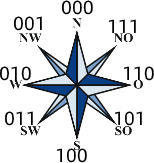
\includegraphics[scale=0.5]{bild12.png}(b)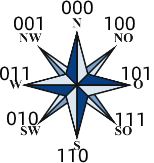
\includegraphics[scale=0.5]{bild11.png}

\noindent\textbf{A2}

Definieren und systematisieren Sie die Begriffe:定义和系统化这些术语:

(a)Binärcode二进制代码

\textbf{Ans:}Codes über dem Alphabet $\{0, 1\}$.

(b)Blockcode区块码

\textbf{Ans:}Codes mit konstanter Codewortlänge.

(c)Linearer Code线性码

\textbf{Ans:}Summe zweier gültiger Codeworte ist ebenfalls ein gültiges Codewort (Modulo-Arithmetik!)

(d)Zyklischer Code循环码

\textbf{Ans:}Durch bitweises Rotieren eines Codewortes entsteht wieder ein gültiges Codewort.

(e)Systematischer Code系统代码

\textbf{Ans:}Codeworte bestehen aus m Informationsbits gefolgt von n-m Prüfbits (Prüfstellen).

\noindent\textbf{A3}

Weisen Sie nach, dass für Lineare Codes gilt证明适用于线性代码

(a)Das Null-Element ist stets ein gültiges Codewort空元素始终是有效的代码字

\textbf{Ans:} Nullelement $\oplus$ ein gültiges Codewort A = ein gültiges Codewort B

(b)Der Minimale Hammingabstand ist gleich dem minimalen Gewicht aller Codeworte, die ungleich Null sind
最小汉明距离等于所有非零代码字的最小权重

\textbf{Ans:}$dist(u,v)=Gewicht(u+v),dist_{min}(u,v)=dist_{u\neq 0}(u,0)=Gewicht_{min}(u)$ 

\noindent\textbf{A4}

Gegeben ist der Code代码给出: $C=\{0000000000, 0000011111, 1111100000, 1111111111\}$

(a)Wieviele Bitfehler sind erkennbar?可识别多少位错误?

\textbf{Ans:}Der Code $C_i$ hat einen Abstand von 5. Damit sind 4 Bitfehler erkennbar.
(Um d Fehler zu erkennen, braucht der Code einen Hammingabstand von d+1. Damit ist es ausgeschlossen, mit d Einzelbitfehlern ein gültiges Codewort zu erhalten)

(b)Wieviele Bitfehler sind korrigierbar?可以纠正多少位错误?

\textbf{Ans:}2 Fehler sicher zu korrigieren.
(Um d Fehler korrigieren zu können, braucht der Code einen Hammingabstand von 2d+1. Damit wird sichergestellt, dass das Fehlerhafte Codewort bei d Fehlern noch immer näher am Originalen Codewort liegt.)

\noindent\textbf{A5}

Lineare Systematische Codes线性系统代码

(a)Codieren Sie die Information 000, 100, 110 und 111 mithilfe der folgenden Generatormatrix:
使用以下生成器矩阵对信息000、100、110和111进行编码:

$$G=(I_k,A)=\begin{bmatrix}
    1&0&0&:&0&1&1\\
    0&1&0&:&1&0&1\\
    0&0&1&:&1&1&0
\end{bmatrix}$$

\textbf{Ans:}$c=x^T\cdot G\Rightarrow 000\cdot G\rightarrow 000000,100\cdot G\rightarrow 100011,110\cdot G\rightarrow 110110,111\cdot G\rightarrow 111000$

(b)Decodieren Sie das empfangene Codewort 001110.解码收到的代码字001110。

\textbf{Ans:}前三位为数据,后三位为校验位。因此代码为:001.

(c)Handelt es sich bei 011011 und 010100 um gültige Codeworte des vorgestelltenCodes?是否提供了011011和010100的有效代码字?

\textbf{Ans:}(1)计算校验矩阵$P=(A^T,I)$,其中$G=(I,A)$,则$\Rightarrow s=P\cdot c^T,P\cdot(011011)^T =(000)^T\checkmark,P\cdot(010100)^T=(001)^T\times$

(d)Wie kann bei dem fehlerhaft empfangenen Codewort 100110 auf die ursprünglich gesendete Information geschlossen werden?
当错误接收到代码字100110时,如何推断原始发送的信息?

\textbf{Ans:}用收到的码乘以校验矩阵P,得到一个校验码,对这个校验码取反(1变0,0变1)得到一个码A,在Nebenklassen表的码A部分选取关键类,将关键类与收到的码异或相加,得到改正的码。

$Syndrom suchen \rightarrow Klasse bestimmen \rightarrow Nebenklassenführer bestimmen \rightarrow Empfangene Nachricht + NK Führer = Korrigiertes Codewort$ 

\section{Ü 4 Codierung 2}

\noindent\textbf{A1}

Zur Absicherung der Datenübertragung in einem Netzwerk existiere ein einfaches Netzwerkprotokoll, welches die Daten zusammen mit einer CRC-Blockprüfzeichenfolge überträgt. Als Generatorpolynom wird $x^3+x+1$ verwendet.
为了确保网络中的数据传输安全,有一个简单的网络协议可将数据与CRC块校验字符串一起传输。 $ x ^ 3 + x + 1 $用作生成多项式

(a)Der Sender möchte die Information 0011 übertragen. Geben Sie das dabei übermittelte Codewort an. 
发送者要发送信息0011。 输入发送的代码字

\textbf{Ans:}(1)根据g(x)参数的幂,可以确定循环码:1011。最高次幂=3,则r=3。

\quad \quad \,\,(2)先求$p(x)=Polynom(0011)$

\quad \quad \,\,(3)求CRC余数:$R(x)=(p(x)\cdot x^r) MOD g(x) = 011$,MOD为模二取余(除法中的加法为异或相加)操作。结果长度应等于r。

\quad \quad \,\,(4)求出c(x),即发送码。$c(x)=(p(x)\cdot x^r)\oplus R(x)=11011$

(b)Handelt es sich bei dem Generatorpolynom um ein primitives Polynom?生成多项式是原始多项式吗?

\textbf{Ans:}Nein. 原始多项式是通过原始信息直接生成的多项式。即p(x)。

(c)Was für Fehler können mit diesem Verfahren erkannt werden?此过程可以检测到哪种错误?

\textbf{Ans:}(1)alle 1-bit-Fehler 

\quad \quad \,\,(2)alle Fehler der Form $e(x) = x^i + x^j = x^i(x^{j-i}+1)$, so lange xj-i+1 nicht von g(x) ohne Rest geteilt wird.
(Für Fall 2 existieren Polynome, die sehr große $j-i$ erlauben. Z.B. $x^{15}+x^{14}+1$ bis zu 32768.)


\quad \quad \,\,(3)alle Fehler mit einer ungeraden Anzahl von Fehlerstellen

\quad \quad \,\,(4)burst-Fehler unterschiedlicher Länge


\noindent\textbf{A2}

Unter Nutzung des in Aufgabe 1 beschriebenen Netzwerkprotokolls erhält ein Empfänger die Übertragung 11101.
使用A1中描述的网络协议,接收器接收传输11101。

(a)Hat die Übertragung fehlerfrei stattgefunden?转移没有错误吗?

\textbf{Ans:}Fehlerfrei. (11101 MOD 1101 = 0)

(b)Welche Information wurde ursprünglich verarbeitet?最初处理了哪些信息?

\textbf{Ans:}不知。

\noindent\textbf{A3}

Ein anderes Netzwerkprotokoll verwendet zur Prüfsummenbildung das CRC-Generatorpolynom $x^4+x+1$. Damit sollen folgende Informationen kodiert werden:
另一个网络协议使用CRC生成多项式$ x ^ 4 + x + 1 $生成校验和。 目的是对以下信息进行编码:

(a)10110

\textbf{Ans:}$g(x)\Rightarrow 10011,r=4,p(x)=x^4+x^2+x,R(x)=(p(x)\cdot x^r)MOD g(x)=1111,c(x)=(p(x)\cdot x^r)\oplus 1111=101101111$

(b)$x^6+x^4+x^2$

\textbf{Ans:}$p(x)\Rightarrow 1010100,R(x)=1110,c(x)=10101001110$

\noindent\textbf{A4}

Stellen Sie ein Schieberegister dar, welches zur technischen Umsetzung des Generatorpolynoms $x^4+x+1$ aus Aufgabe 3 dient. Benutzen Sie dieses Schieberegister, um die Information 1101 zu codieren.
表示一个移位寄存器,用于技术执行任务3的生成多项式$ x ^ 4 + x + 1 $。 使用此移位寄存器对信息1101进行编码。

\textbf{Ans:}

\quad \quad \,\,(1)根据g(x)得到的CRC码,画出硬件设计如图。(D为DFF)

任意CRC电路图如图所示:
\begin{center}
    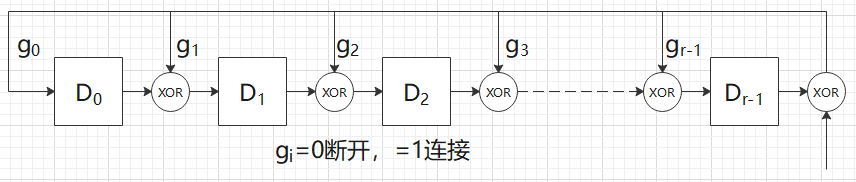
\includegraphics[scale=0.4]{bild13.png}
\end{center}

\indent\indent 已知$g(x)=x ^ 4 + x + 1 \Rightarrow 10011$, r=4, 则有4个DFF。$g_0=1, g_1=1, g_2=0, g_3=0$。

\indent\indent 则有电路图:

\begin{center}
    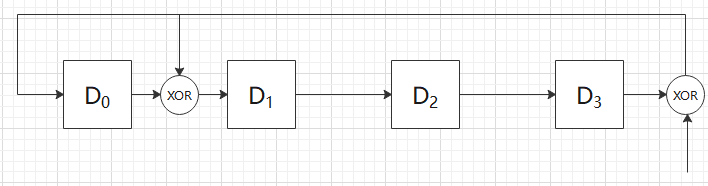
\includegraphics[scale=0.4]{bild14.png}
\end{center}

\quad \quad \,\,

\quad \quad \,\,(2)计算(最终在DFF中的数据$d_0d_1d_2d_3$就是余值(CRC-Rest)):

\begin{center}
    \begin{tabular}{c|c|c|c|c|c|c}
        Eingabe(folge)&$D_0$&$D_1$&$D_2$&$D_3$&Ausgabe&\\
        \hline
        待定
    \end{tabular}
\end{center}

\section{Ü 5 Codierung 3}

\noindent\textbf{A1}

ISO/OSI-Modell

a) Was sind die Vorteile eines schichtenartigen Kommunikationsmodells?分层通信模型的优点是什么?

b) Was versteht man unter horizontaler und vertikaler Kommunikation zwischen Schichten?层之间的水平和垂直通信是什么?

c) Nennen Sie wesentliche Aufgaben der Sicherungsschicht im ISO/OSI-Modell.在ISO / OSI模型中命名数据链路层的基本任务。

\textbf{Ans:}

\textbf{a)}

\indent\indent (1)Es unterteilt die Netzkommunikation in kleinere, einfacher zu handhabende Teile.
它将网络通信分为较小的,易于使用的部分。

\indent\indent (2)Es standardisiert Netzkomponenten, um die Entwicklung und Unterstützung durch verschiedene Hersteller zu ermöglichen.
它使网络组件标准化,以支持各种制造商的开发和支持。

\indent\indent (3)Es ermöglicht die Kommunikation zwischen unterschiedlicher Netzhardware und –software.
它支持不同网络硬件和软件之间的通信。

\indent\indent (4)Es verhindert, dass Änderungen auf einer Schicht die übrigen Schichten beeinflussen.
它可以防止一层上的更改影响其他层。

\indent\indent (5)Es unterteilt die Netzkommunikation in kleinere Teile, um sie leichter verständlich zu gestalten.
它将网络通信分成较小的部分,以使其更易于理解。

\textbf{b)}

\begin{center}
    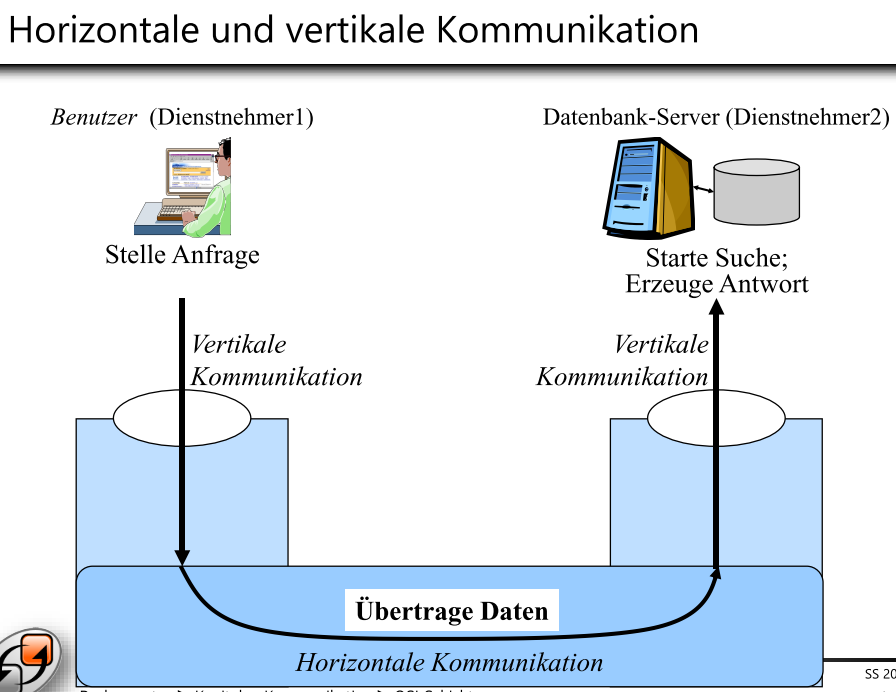
\includegraphics[scale=0.4]{bild15.png}
\end{center}

\textbf{c)}

定义了如何让格式化数据以进行传输,以及如何让控制对物理介质的访问。这一层通常还提供错误检测和纠正,以确保数据的可靠传输。
Definiert, wie Daten für die Übertragung formatiert und der Zugriff auf physische Medien gesteuert werden. Fehlererkennung und -korrektur.

\noindent\textbf{A2}

Sicherungsschicht数据链路层

\textbf{a)} Was versteht man unter Codetransparenz und wie kann diese erreicht werden?什么是代码透明性,如何实现?

b) Was passiert mit Paketen, die fehlerhaft beim Empfänger ankommen?错误地到达收件人的包裹会发生什么?

c) Geben Sie ein Beispiel für geregelten und konkurrierenden Zugriff auf ein Übertragungsmedium an.
举例说明对传输介质的管制访问和竞争访问。

d) Was ist die Grundidee hinter CSMA/CD?CSMA / CD的基本思想是什么?

e) Was sind MAC-Adressen?什么是MAC地址?

\textbf{Ans:}

\textbf{a)}Vereinbarung von Regeln zur codetransparenten Übertragung von Nutzdaten (d.h. Übertragung beliebiger Bit- bzw. Zeichenkombinationen im Nutzdatenfeld).

\textbf{b)}Der Empfänger prüft auf Fehler und fordert eine erneute Übertragung an. 接收方检查错误并要求重新传输。

\textbf{c)}

\begin{center}
    \begin{tabular}{c|c}
        Geregelter Zugriff&Konkurrierender Zugriff\\
        \hline
        HDLC(im Aufforderungsbetrieb)&Aloha/Slotted Aloha\\
        Token-Ring, Token Bus&Ethernet(CSMA,CSMA/CD)\\
        FDDI
    \end{tabular}
\end{center}

\textbf{d)}所有站以相同的权限连接到同一总线。当媒体显示空闲时,任何电台都可以发送。
Alle Stationen gleichberechtigt an gemeinsamen Bus angeschlossen. 
Jede Station kann senden, wenn Medium frei erscheint.

\textbf{e)}Die MAC-Adresse (Media-Access-Control-Adresse) ist die Hardware-Adresse jedes einzelnen Netzwerkadapters, die als eindeutiger Identifikator des Geräts in einem Rechnernetz dient.

\noindent\textbf{A3}

Ethernet以太网络

a) Aus was für Feldern besteht der Header eines Ethernet II –Framesund was machen sie? 以太网II帧的标头包含哪些字段,它们做什么?

b) Wie kann man eine Nachricht an alle erreichb.Rechner in einem lokalen Netzwerk senden?如何将消息发送到局域网中的所有可访问计算机?

c) Warum muss ein Ethernetframe eine minimale Größe besitzen und wie groß ist diese?为什么以太网帧必须具有最小尺寸,该尺寸有多大?

\textbf{Ans:}

\textbf{a)}

\begin{center}
    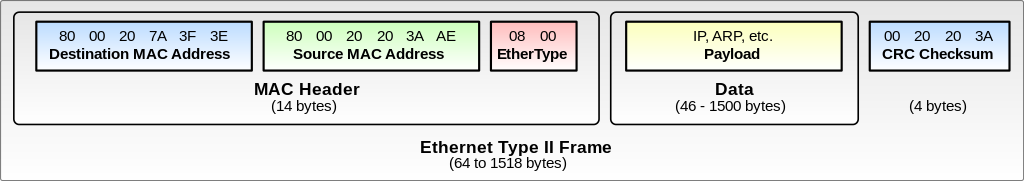
\includegraphics[scale=0.4]{bild16.png}
\end{center}

\textbf{b)}

Lookup-Tabelle,Berechnung,Nachrichtenaustausch.

Praktisch wird Nachrichtenaustausch (Address Resoultion Protocol) verwendet.

\textbf{c)}Minimale Rahmengröße von 64 Byte, maximal 1500 Byte.

参见上方Ethernet II以太网帧格式可知:目标MAC 6字节 + 源MAC 6字节 + Type 2字节 + 数据 46-1500字节 + 校验位 4字节=64-1518。
(注:ISL封装后可达1548字节,802.1Q封装后可达1522字节)

\noindent\textbf{A4}

Switch交换机

a) Wie funktioniert ein Switch im Gegensatz zu einem Repeater / Hub?与中继器/集线器相比,交换机如何工作?

\textbf{Ans:}(1)Analysiert Netzverkehr und trifft logische Entscheidungen $\rightarrow$ intelligenter Hub

\indent\indent(2)Ports können unabhängig voneinander Daten empfangen und senden

\indent\indent(3)verarbeitet bei Erhalt eines Pakets die MACAdresse und legt zusammen mit dem physikalischen Port einen Eintrag in der SAT (Source-Address-Table) an.

\indent\indent(4)wenn Zieladresse noch unbekannt $\rightarrow$ Weiterleitung an alle aktiven Ports

b) Wie verhindert das Spanning Tree Protokoll endlos kreisende Daten in einem lokalen Netzwerk mit redundanten Wegen?
生成树协议如何防止具有冗余路径的本地网络中的数据不断循环?

\textbf{Ans:}Er identifiziert Mehrfachwege, indem er Topologien mit redundanten Wegen durch eine logische Blockierung bestimmter Pfade in eine Baumtopologie überführt, die keine Schleifen besitzt. Dazu werden auf den Switches mit mehreren Verbindungen zu anderen Switches alle bis auf eine Verbindung blockiert. Bei Ausfall der primären Verbindung können diese sofort aktiviert werden und erzeugen auf diese Weise ein hohes Maß an Fehlertoleranz.
任意一交换机中如果到达根网桥有两条或者两条以上的链路,生成树协议都根据算法把其中一条切断,仅保留一条,从而保证任意两个交换机之间只有一条单一的活动链路。因为这种生成的拓扑结构,很像是以根交换机为树干的树形结构,故为生成树协议。

\section{Ü 6 Statisches Routing}

\noindent\textbf{A1}

Warum reichen MAC-Adressen nicht aus, um weltweit Informationen zwischen zwei beliebigen verbundenen Hosts auszutauschen?
为什么MAC地址不足以在全球任何两个连接的主机之间交换信息?

\textbf{Ans:}见Ans 2012 - A3

\noindent\textbf{A1-补充}

Will ein Rechner mit IP A eine Nachricht an Rechner mit IP B schicken, so geschieht folgendes:
如果具有IP A的计算机要向具有IP B的计算机发送消息,则会发生以下情况:

1. A sendet Broadcast an alle Rechner im Subnetz mit der Anfrage who-has B

2. B sendet Unicast an A I-AM B

\noindent\textbf{A2}

In welchem Netz befindet sich der Rechner mit der IP-Adresse 192.168.1.188 bei der Netzmaske 255.255.255.224 oder /27? 
IP地址为192.168.1.188且网络掩码为255.255.255.224或/ 27的计算机在哪个网络中?

Welche Adressen sind in diesem Netzwerk an einen beliebigen Host vergebbar?哪些地址可以分配给该网络中的任何主机?

\textbf{Ans:}

\begin{center}
    \begin{tabular}{c|c|c}
        Address&192.168.1.188&11000000.10101000.00000001.10111100\\
        Netmask&255.255.255.224/27&11111111.11111111.11111111.11111110\\
        $\Rightarrow$&&将两个二进制地址进行与运算(即只有1与1=1)\\
        Network&192.168.1.188&11000000.10101000.00000001.10111100
    \end{tabular}
\end{center}

\begin{center}
    \begin{tabular}{c|c|c|c|c|c}
        Class&IP最高位&子网掩码&范围&可分配主机个数&可分配网络数\\
        A&0&255.0.0.0&0.0.0.0 - 127.255&$2^{24}-2$&$2^7-2$\\
        B&10&255.255.0.0&128.0.0.0 - 191.255&$2^{16}-2$&$2^{14}-1$\\
        C&110&255.255.255.0&192.0.0.0 - 233.255&$2^{8}-2$&$2^{21}-1$
    \end{tabular}
\end{center}

\indent 广播地址的最后一段数字永远是255,此题的Boardcast:192.168.1.255

\indent Host: 192.168.1.0

\indent 对于此题,与运算(可分配的地址,子网掩码255.255.255.224)=192.168.1.188即可。即还可以分配192.168.1.189。

\noindent\textbf{A3}

Bestimmen Sie die Routingtabellen auf Router 1 bis 3. 确定路由器1到3上的路由表

\begin{center}
    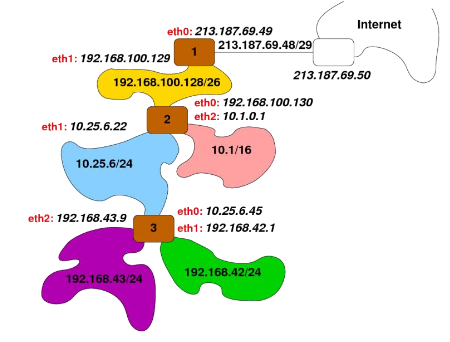
\includegraphics[scale=0.6]{bild9.png}
\end{center}

\textbf{Ans:}

计算方法:Ziel写任意主机地址,Netzmaske为该主机所在网络,Gateway网关写下一跳服务器出口,Interface接口写最终跳服务器入口。

R3的路由表:
\begin{center}
    \begin{tabular}{c|c|c|c}
        Ziel&Netzmaske&Gateway&Interface\\
        \hline
        213.187.69.48&255.255.255.248&10.25.6.22&eth0\\
        192.168.100.128&255.255.255.192&10.25.6.22&eth0\\
        10.1.0.0&255.255.0.0&10.25.6.22&eth0\\
        10.25.6.0&255.255.255.0&*&eth0\\
        192.168.43.0&255.255.255.0&*&eth2\\
        192.168.42.0&255.255.255.0&*&eth1\\
        default&0.0.0.0&10.25.6.22&eth0
    \end{tabular}
\end{center}

\section{Ü 7 Dynamisches Routing}

\noindent\textbf{A1}

Wann sind statische Routingverfahren nachteilig?静态路由方法何时不利?

\textbf{Ans:}

Manuelle Pflege von Routingeinträgen nicht immer sinnvoll:

\indent \indent Wenn Routing Redundanz schaffen soll.

\indent \indent Wenn Netz sehr groß ist.

\indent \indent Wenn Netz sehr oft Änderungen unterworfen ist.

\noindent\textbf{A1-补充1}

Automatische Routingprotokolle greifen auf zwei verschiedene Ansätze zurück自动路由协议使用两种不同的方法:

\indent \indent distance vector (z.B. RIP)

\indent \indent link state (z.B. OSPF)

\noindent\textbf{A1-补充2}

\textbf{Distance Vector} 包含:(1)Berechnen Routing verteilt. (2)Bellman Ford Algorithmus. (3)Periodischer Austausch von Distanz-Vektoren.

Bellman Ford Algorithmus:

\indent \indent Jeder Knoten kennt initial nur die Kosten zu seinen direkten Nachbarn
每个节点最初只知道其直接邻居的成本。

\indent \indent Jeder Knoten pflegt Tabelle mit möglichen Zielen, den Gesamtkosten zu diesem Ziel und den namen der ersten Station
每个节点维护一个表,其中包含可能的目的地,该目的地的总费用以及第一个站点的名称。

\indent \indent Jeder Knoten schickt sein Wissen periodisch an alle Nachbarn
每个节点定期将其知识发送给所有邻居。

\indent \indent Ein Knoten, der Informationen erhält, aktualisiert seine Tabelle
接收信息的节点更新其表。

\indent \indent (Aktualisieren bedeutet: Ist noch keine Information über Ziel bekannt, dann Information speichern. Ist Information bekannt, dann prüfen, ob neue Information eine günstigere Strecke ermöglicht.更新意味着:如果不知道有关目的地的信息,则保存信息。 如果知道信息,请检查新信息是否使路由更便宜。)

\noindent\textbf{A2}

Welche Probleme können  bei Distanz-Vektor-Protokollenauftreten?距离矢量协议会出现什么问题?

\textbf{Ans:}

(1)Langsame Konvergenz

(2)Bei gewichteten Links können Routing-Schleifen entstehen

(3)Sehr langsame Propagierung von Kostensteigerungen oder Ausfällen

\indent\indent(其中的Kostensteigerungen:Knoten K hat Knoten N als Anfang einer kürzesten Strecke zu X. Erhöhen sich bei N die Kosten zu X, dann teilt dieser das auch K mit. K muss wiederum seine Kosten anpassen, wenn er lernt, dass es zu X über N nun teuerer geworden ist.)

\indent\indent(其中时间问题Count to infinity durch ungeschicktes Timing.解决办法:Split horizon)

\noindent\textbf{A3}

Was sind Vorteile und Nachteile von Link State Routing –Protokollen im Vergleich zu Distanz-Vektor-Protokollen?
与距离矢量协议相比,链路状态路由协议的优缺点是什么?

\textbf{Ans:}

\begin{center}
    \begin{tabular}{c|c}
        Vorteile&Problem Heute\\
        \hline
        Konvergiert schneller als RIP&AS-Nummern werden knapp\\
        keine Routing Loops&Hoher Speicherverbrauch\\
        mehrere Metriken parallel\\
        Lastverteilung auf mehrere Pfade
    \end{tabular}
\end{center}


\noindent\textbf{A4}

Gegeben ist eine Menge von sieben Routern, welche sich entsprechend nachstehender Abbildung gegenseitig erreichen können
有一组七个路由器,可以根据以下插图相互连接

\begin{center}
    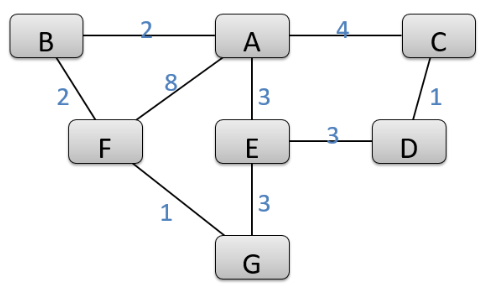
\includegraphics[scale=0.5]{bild10.png}
\end{center}

Bestimmen Sie unter Verwendung des OSPF-Protokolls.确定使用OSPF协议

a)die kürzeste Route von A nach G

b)die kürzeste Route von B nach D?

\textbf{Ans:}

解决方法:Benutzt Dijkstras Algorithmus zur Bestimmung kürzester Wege使用Dijkstra的最短路径算法
(BFS)

Jeder Knoten kennt alle Verbindungen im Netz每个节点都知道网络中的所有连接

von A nach G:

\begin{center}
    \begin{tabular}{c|c|c|c|c|c|c|c}
        &A&B&C&D&E&F&G\\
        \hline
        初始&0&$\infty$&$\infty$&$\infty$&$\infty$&$\infty$&$\infty$\\
        \hline
        找到A相连的节点&&2,A&4,A&&3,A&8,A\\
        \hline
        选取上面路径最短的节点,为B&&&&&&4,B\\
        \hline
        同理,选E&&&&6,E&&&6,E\\
        \hline
        选C&&&&5,D&&&\\
        \hline
        选F&&&&&&&5,F
    \end{tabular}
\end{center}

得到最短路径$A\rightarrow G \Rightarrow A\rightarrow B\rightarrow F\rightarrow G$

\noindent\textbf{A5}

Ist eine IP-Adresse in einem Subnetz nicht vorhanden, wird das Paket an ein definiertes Standardgateway weitergeleitet, welches es weitervermittelt. Jedoch kann es passieren, dass es die Empfängeradresse weltweit gar nicht gibt. Was passiert indiesem Fall?
如果子网中没有IP地址,则将数据包转发到转发的已定义标准网关。 但是,可能会发生收件人地址不存在全世界的情况。 在这种情况下会发生什么?

\textbf{Ans:}IP hat TTL(Time to live). Wenn ein Datenpaket nach Ablauf seiner TTL noch nicht sein Ziel erreicht hat, wird es verworfen.

\section{Ü 8}

\noindent\textbf{A1}

a)Welche Dienste werden im ISO/OSI-Referenzmodell auf der Transportschicht erbracht?传输层上的ISO / OSI参考模型提供了哪些服务?

\textbf{Ans:}

\indent \indent Anwendungsmultiplexing / -adressierung 

\indent \indent Einheitlicher Zugriff auf Kommunikationsnetz 

\indent \indent Kommunikationssteuerung 

\indent \indent Zuverlässige Datenübertragung (TCP) 

\indent \indent Überlastkontrolle

b)Was wird auf der Transportschicht zur Adressierung verwendet und wofür?在传输层上用于寻址的内容是什么?

\textbf{Ans:}IP

c)Was sind Sockets?什么是Sockets?

\textbf{Ans:}standardisierte Programmierschnittstelle (API) für Anwendungen, um die Netzwerkprotokoll-Implementierung des Betriebssystems zu nutzen.

d)An was für einem TCP-Standardport lauscht in der Regelein Webserver-Prozess?Web服务器进程正在侦听哪种类型的标准TCP端口?

\textbf{Ans:}80

e)Was für eine Anwendung wird in der Regel an den TCP-Standardport 25 gebunden?标准TCP端口25通常绑定哪种应用程序?

\textbf{Ans:}E-Mail Versand

\textbf{A1-补充:}

\begin{center}
    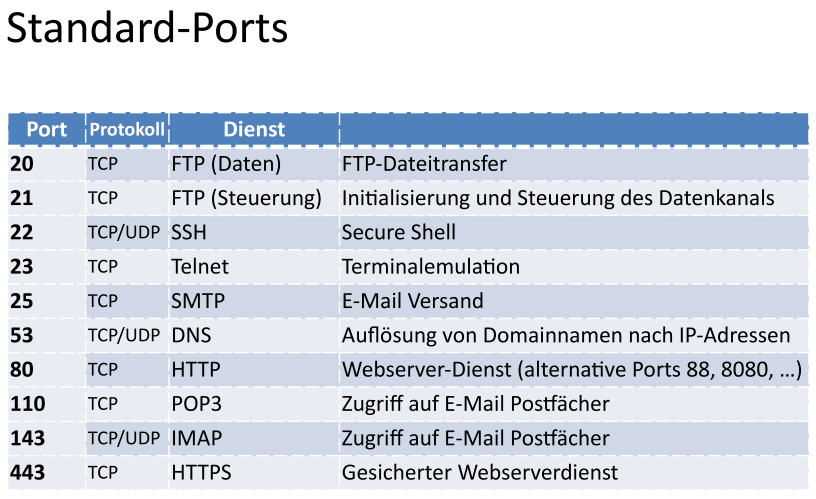
\includegraphics[scale=0.5]{bild17.png}
\end{center}

\noindent\textbf{A2}

a)Schreiben Sie ein Programm in Python für einen Serverdienst, der auf einem PC lokal läuft, via UDP an Port 1470 eine Textnachricht entgegennimmt und diese Nachricht anschließend mit +++ -Zeichen umschlossen zurück an den Client sendet.
用Python编写一个用于在PC上本地运行的服务器服务的程序,通过UDP在端口1470上接收文本消息,然后将此消息发送回客户端,并用+++字符括起来

b)Schreiben Sie ebenso ein Python-Script für einen Client, der via UDP den Text „Hello world“ an den Server aus Aufgabenteil a sendet und dessen Antwort empfängt und auf der Kommandozeile ausgibt.
还为客户端编写Python脚本,该客户端通过UDP从任务部分a向服务器发送文本“ Hello world”到服务器,并接收其响应并将其输出到命令行。

c)Wie müssen die Skripte aus 2a und 2b verändert werden, wenn die Kommunikation via TCP erfolgen soll?
如果要通过TCP进行通信,如何更改2a和2b中的脚本?

\noindent\textbf{A3}

Ein Client initiiert unter Verwendung von TCP einen 3-way-Handshake mit einem Server, indem er ein SYN mit der zufälligen Sequenznummer 91 sendet. Wie sieht die weitere Kommunikation zwischen den beiden Kommunikationspartnern aus? Was hat das für einen Zweck?
客户端通过发送带有随机序列号91的SYN,使用TCP与服务器启动3way握手。 两个交流伙伴之间的进一步交流看起来如何? 什么目的?

\textbf{Ans:}Der Zweck besteht darin, die Seriennummer und die Bestätigungsnummer beider Parteien zu synchronisieren und Informationen zur TCP-Fenstergröße auszutauschen.

\begin{center}
    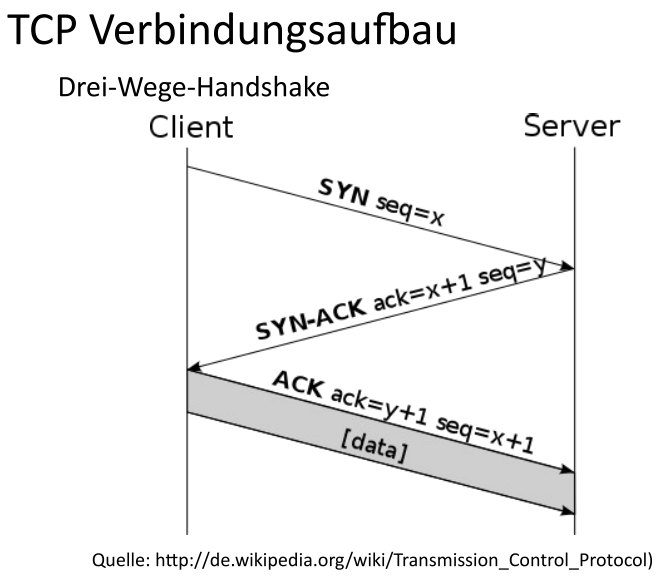
\includegraphics[scale=0.5]{bild18.png}
\end{center}



\section{Ü 9}

\noindent\textbf{A1}

a)Wie lautet ein HTTP-Request, um von dem Server  www.tu-chemnitz.de  die  Datei informatik.html abzurufen? 
从服务器www.tu-chemnitz.de获取文件informatik.html的HTTP请求是什么?

\textbf{Ans:}GET https://www.tu-chemnitz.de/informatik.html HTTP/1.1

b)Was ist der Unterschied zwischen den HTTP-Methoden GET und POST? HTTP方法GET和POST有什么区别?

\textbf{Ans:}
\begin{center}
    \begin{tabular}{c|c}
        GET&POST\\
        \hline
        \shortstack[l]{Der Browser sendet den http-Header und \\
        die Daten zusammen und der Server\\
         antwortet mit 200 (Daten zurückgeben).}&\shortstack{Der Browser sendet zuerst den Header, \\
         der Server antwortet mit 100 Weiter, \\
         der Browser sendet erneut Daten und der \\
         Server antwortet mit 200 OK (Daten zurückgeben).}
        
    \end{tabular}
\end{center}


c)Was besagen die HTTP Response-Codes 200, 404 und 500? HTTP响应代码200、404和500是什么意思?

\textbf{Ans:}

\indent\indent 200: alles in Ordnung, gewünschte Daten folgen.

\indent\indent 404: URL nicht gefunden, statt Daten meist Fehlerbeschreibungsseite.

\indent\indent 500: Internal Server Error

其他见附件表

d)Sie geben in Ihrem Webbrowser die URL einer Webseite mit Bildern ein. Beschreiben Sie die Lade-Vorgänge auf dem Netz. 
您在网络浏览器中输入带有图像的网站的URL。 描述网络上的计费过程。

\textbf{Ans:}

e)Was bedeutet bei HTTP/1.1 Keep-Alive? 

\textbf{Ans:}Ein Keep Alive ist ein Signal, das von einem Gerät zu einem anderen gesendet wird, um eine Verbindung zwischen den beiden Geräten aufrechtzuerhalten. 

f)Warum  muss  bei  einem  HTTP/1.1-Request zwingend  das  Headerfeld  Host  angegeben werden? 
为什么必须为HTTP/1.1-Request指定Host标头字段?

\textbf{Ans:}Wenn mehrere Websites auf einem Server bereitgestellt werden, wird es durch den Host-Request entscheidet , welche Website  besucht werden soll.

\noindent\textbf{A2}

Beschreiben Sie den Protokollablauf, wie ein E-Mailprogramm unverschlüsselt.将协议流描述为未加密的电子邮件程序 

a)Ihre Mailbox auf neue E-Mails mittels POP3 überprüft. 使用POP3检查邮箱中是否有新电子邮件

b)eine neue-Email an Ihren E-Mailanbieter via SMTP übermittelt.通过SMTP向您的电子邮件提供商发送了一封新电子邮件。

\noindent\textbf{A3}

Um  eine  Webdomain  zu  einer  IP-Adresse  des Webservers aufzulösen, wird DNS verwendet. 
DNS用于将Web域名解析为Web服务器的IP地址。

a)Was ist ein FQDN? 

b)Was ist ein Nameserver? 

c)Was  ist  der  Unterschied  zwischen  einer rekursiven und einer iterativen DNS-Abfrage?
递归和迭代DNS查询有什么区别?

\textbf{Ans:} a) b)见Ans2016 - A7

\textbf{c)}

rekursiven DNS-Abfrage: Der DNS-Server als DNS-Client fragt diese Auflösungsanforderung von anderen DNS-Servern ab, bis das Auflösungsergebnis erhalten wird.

iterativen DNS-Abfrage: Der DNS-Server stellt dem Client andere DNS-Serveradressen zur Verfügung, mit denen die Abfrageanforderung aufgelöst werden kann. Wenn der Client die Abfrageanforderung sendet, antwortet der DNS-Server nicht direkt auf das Abfrageergebnis, sondern teilt dem Client eine andere DNS-Serveradresse mit. Dieser DNS-Server sendet die Anforderung und wiederholt die Schleifen, bis das Ergebnis der Abfrage zurückgegeben wird.

\end{document}